%%==================================================
%% diss.tex for SJTU Bachelor Thesis
%% based on CASthesis
%% version: 0.3a
%% Encoding: UTF-8
%%==================================================

% 字号选项: c5size 五号(默认) cs4size 小四
% 双面打印(注意字号设置)
%\documentclass[cs4size, a4paper, twoside]{sjtuthesis} 
% 单面打印(注意字号设置)

\expandafter\def\csname CTEX@spaceChar\endcsname{\hspace{1em}}
\documentclass[cs4size, a4paer, oneside, openany]{sjtuthesis} 

\CTEXsetup[name={,},number=\arabic{chapter}]{chapter}

\usepackage[titles]{tocloft}
\renewcommand{\cftchapfont}{\normalfont}
\renewcommand{\cftchappagefont}{\normalfont}

\usepackage[english]{babel}
\usepackage{english_chapter}
\usepackage{csquotes}

\usepackage{fmtcount,etoolbox}
\makeatletter
\patchcmd{\@makechapterhead}{\thechapter}{\Numberstring{chapter}}{}{}
\makeatother

\setcitestyle{citesep={;},aysep={,},yysep{;},notesep={: }}
\newcommand{\ifempty}[3]{\ifx\something#1\something{#2}\else{#3}\fi}
\newcommand{\sjtucite}[2][]{([{\citenum{#2}}], \citeauthor{#2}, \citeyear[#1]{#2}\ifempty{#1}{}{: #1})}

% \usepackage[sectionbib]{chapterbib}%每章都用参考文献
\usepackage{setspace}
\newboolean{DOIT}
\setboolean{DOIT}{false}%编译某些只想自己看的内容,编译true,否则false

%% 行距缩放因子(x倍字号)
\renewcommand{\baselinestretch}{1.3}

% 设置图形文件的搜索路径
\graphicspath{{figure/}{figures/}{logo/}{logos/}{graph/}{graphs}}

\newcommand{\argmax}{\operatornamewithlimits{argmax}}
\newcommand\vu{\mathbf{u}}
\newcommand\vw{\mathbf{w}}
\newcommand\vz{\mathbf{z}}
\newcommand\vd{\mathbf{d}}
\newcommand\va{\mathbf{a}}
\newcommand\vr{\mathbf{r}}
\newcommand\vh{\mathbf{h}}
\newcommand\vm{\mathbf{m}}
\newcommand\RNN{\mathbf{RNN}}
\newcommand\sims{\text{sim}}


%%========================================
%% 在sjtuthesis.cls中定义的有用命令
%%========================================
% \cndash 中文破折号
% 数学常量
% \me 对数常数e
% \mi 虚数单位i
% \mj 虚数单位j
% \dif 直立的微分算符d为直立体。
% 可伸长的数学箭头、等号
% \myRightarrow{}{}
% \myLeftarrow{}{}
% \myBioarrow{}{}
% \myLongEqual{}{}
% 参考文献
% \upcite{} 上标引用
%%========================================


\begin{document}

\setlength\parindent{0pt}

%%%%%%%%%%%%%%%%%%%%%%%%%%%%%% 
%% 封面
%%%%%%%%%%%%%%%%%%%%%%%%%%%%%% 

% 中文封面内容(关注内容而不是形式)
\title[Multistage Clustering Method]{for Unsupervised Aspect Mining}{\normalsize Multistage Clustering Method for Unsupervised Aspect Mining}
\author{冯实}
\advisor{朱其立}
\degree{学士}
\defenddate{}
\school{上海交通大学}
\institute{致远学院}
\studentnumber{5120719013}
\major{计算机科学与技术(交大ACM班)}

% 英文封面内容(关注内容而不是表现形式)
\englishtitle{Multistage Clustering Method for Unsupervised Aspect Mining}
\englishauthor{Shi Feng}
\englishadvisor{Prof. Kenny Q. Zhu}
\englishschool{Shanghai Jiao Tong University}
\englishinstitute{Zhiyuan College}
\englishdegree{Bachelor}
\englishmajor{Computer Science and Technology (SJTU ACM Class)}
\englishdate{}

% 封面
\maketitle

% 英文封面
%\makeenglishtitle

% 论文原创性声明和使用授权
%\makeDeclareOriginal
%\makeDeclareAuthorization

%%%%%%%%%%%%%%%%%%%%%%%%%%%%%% 
%% 前言
%%%%%%%%%%%%%%%%%%%%%%%%%%%%%% 
\frontmatter
\pagenumbering{gobble}

% 摘要
%\begin{abstract}
%  In the age of information explosion, search engines have been an
%  essential tool in people's daily life and query suggestion is one
%  of most useful feature for a standard search engine. However, because
%  most of search engines are keyword-based, many fantastic features would
%  fail when facing concept-based queries, so does query suggestion. In this
%  paper, we propose a framework so that search engines can give acceptable
%  suggestions when facing concept-based queries.
%\end{abstract}

\begin{abstract}
  A class of search queries which contain abstract concepts are studied in
this paper. These queries cannot be correctly interpreted by traditional keyword-based search engines.
  This paper presents a simple framework that detects and instantiates the
abstract concepts by their concrete entities or meanings to produce alternate
queries that yield better search results.
\footnote{Kenny Q. Zhu (corresponding author) is partially
supported by NSFC grants 61100050 and 61033002.}
\end{abstract}

\begin{abstract}
情感分析与观点挖掘作为自然语言处理的一个子领域,相比其他领域如信息挖掘,更着重对于自然语言中观点的表达与理解的研究。文档中观点的自动总结是情感分析与观点挖掘中很重要的一个任务。由于网络上用户评论的数目急剧增加,而我们又没有一个统一的总结这些观点的框架和格式,人们现在很关系如何能够自动的从没有结构的数据中挖掘出有结构的知识。其中一种很实用的总结的格式被是围绕方面的观点总结,这种格式常见于TripAdvisor.com等网站,用户除了写文字以外,还会对酒店等产品的各个方面进行打分。在本文中,我们关注如何能够自动的为一个产品找到这些合适的方面,使得我们可以围绕这些方面来总结用户的观点,这个任务称为方面词提取。由于互联网上产品的种类繁多,为每一类产品人工的制定这些方面词是不可行的。而另一方面我们又有大量的无标注的用户评论数据,适于使用非监督机器学习的方法。在本文中,我们提出一种非监督的多阶段聚类框架来解决方面词提取这一问题,其中使用到聚类、话题模型和深度学习及神经网络在自然语言上的应用。我们提出的模型可以很容易的应用到任何领域的数据上,而且不需要任何标注,具有很好的可扩展性。在试验中,我们的模型取得了比其他单阶段方法更好的表现。我们还会展示如何扩展我们的模型,通过搭配情感预测实现一个完整的评论总结。对比诸多电商网站现有的评论总结形式,我们的方法可以提供更清晰、更易比较、更忠实于用户观点的信息。

\keywords{自然语言处理,情感分析,观点挖掘,文档总结,话题模型,深度学习,神经网络,基于方面的观点挖掘}
\end{abstract}


% 目录
\tableofcontents
% 表格索引
\listoftables
% 插图索引
\listoffigures

% \addcontentsline{toc}{chapter}{\listfigurename} %将表格索引加入全文目录
% \addcontentsline{toc}{chapter}{\listtablename}  %将图索引加入全文目录

% 主要符号、缩略词对照表
% \include{body/symbol}

%%%%%%%%%%%%%%%%%%%%%%%%%%%%%% 
%% 正文
%%%%%%%%%%%%%%%%%%%%%%%%%%%%%% 
\mainmatter

%% 各章正文内容
\section{Introduction}
\label{sec:intro}

Evaluation of dialogue systems is an open question. Existing
automatic evaluation metrics for chitchat systems are similar to those for 
other text generation tasks (e.g., machine translation \citep{papineni-etal-2002-bleu}, question-answering \citep{rajpurkar-etal-2016-squad}, 
summarization \citep{lin-2004-rouge}), which depends on calculating word overlaps with 
ground truth reference responses. 
However, for chitchat tasks, there are usually 
many alternative but plausible responses given a situation, 
perhaps more than any other text generation task mentioned above. 
A limited number of reference responses are 
not sufficient to determine how good a generated response is. 
Moreover, such static settings are not good at
assessing an interactive, context-sensitive system.

Interactive human evaluation metrics usually 
involve a Likert scale evaluation after a multi-turn conversation 
with the evaluated bot. 
While this method is a step up from the previous static evaluation, 
it is difficult for human judges to give a concrete score to
any bot.
%\KZ{But are we also asking judges to score invidividual bots, which is difficult?} 
To compare the performance of two bots is easier. 
Thus ACUTE-EVAL~\citep{DBLP:journals/corr/abs-1909-03087} asks the 
judges to make a binary judgment of who is better in conversations between two identical bots 
or between a human and a bot. A more advanced version of that
is \textit{Spot The Bot}~\cite{deriu-etal-2020-spot} which models the 
human evaluation of a 
conversation after the Turing test. Such a process is still 
time-consuming and costly, 
compared with automatic evaluations.

In our opinion, a good method for evaluating multi-turn conversational model/system 
should satisfy the following requirements:
i) be as efficient and inexpensive as possible;
ii) can truly reflect a model's ability to conduct a human conversation; 
iii) evaluation results should correlate well with human judgments;
iv) can be used to compare and rank the capabilities of a set of models/systems.
  
Toward that goal, in this work, we propose an automatic interactive evaluation framework, 
which is called \textit{ChatMatch} for chitchat
agents. This framework can be used to rank any number of bots with very little
time and effort.  Above all, we want to emphasize the significance of
the observation on direct interactions between bots in the evaluation. 
People tend to believe that human-bot conversations are more reliable 
and produce more comprehensive evaluations of chatbots' capabilities. 
This is not always true. As human annotators know their counterpart is a robot, 
they tend to ask common and goal-directed questions. 
The bot-bot chat logs in our experiments show that, surprisingly,  
talking between two different bots may expose both their strengths and weaknesses not seen
in human-bot conversations. 
Here, we take as an example in \figref{fig:two convs} two small fragments 
from the chat logs between humans-bot and bot-bot. While talking about hobbies, 
human keeps asking the bot direct questions, which leads to boring responses from the bot.
However, in a bot-bot setting, two bots, including the same bot in the previous
conversation, start explaining their hobbies to each other, producing a much more natural and 
interesting conversation. 

\begin{figure}[ht!]
\begin{subfigure}{0.5\textwidth}
  \centering
  % include first image
  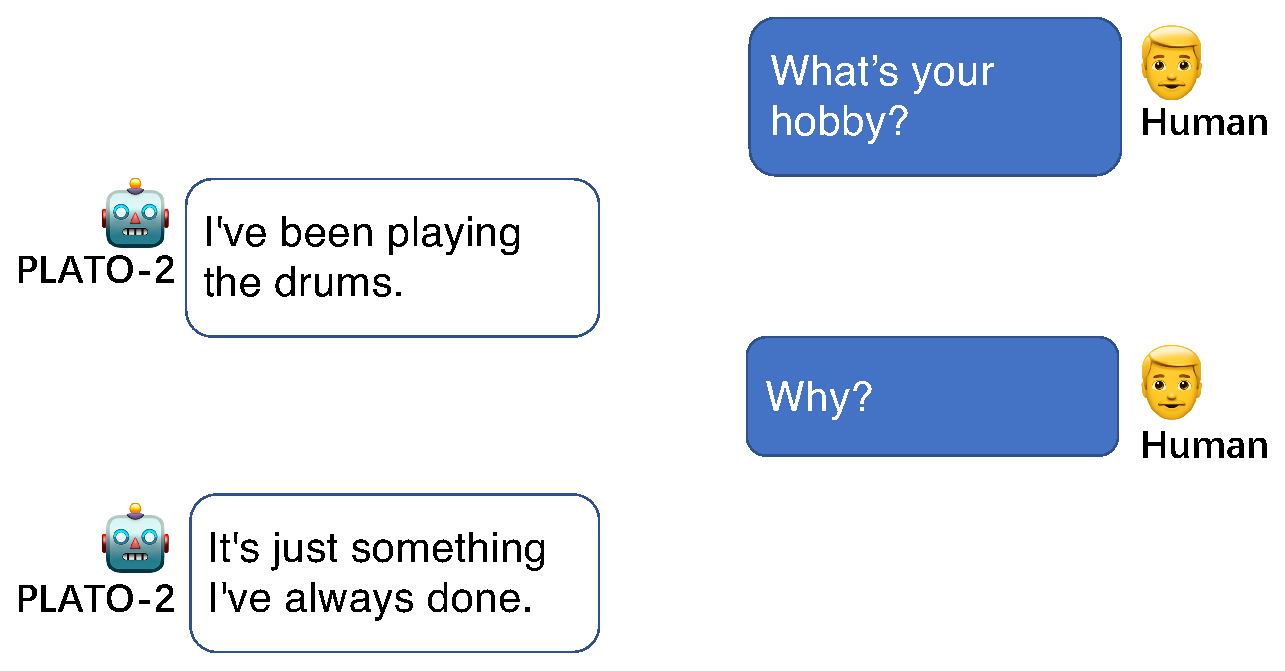
\includegraphics[width=.8\linewidth]{crop1.eps}  
  \caption{A small fragment of conversation between human and bot}
  \label{fig:sub-first}
\end{subfigure}
\begin{subfigure}{0.5\textwidth}
  \centering
  % include second image
  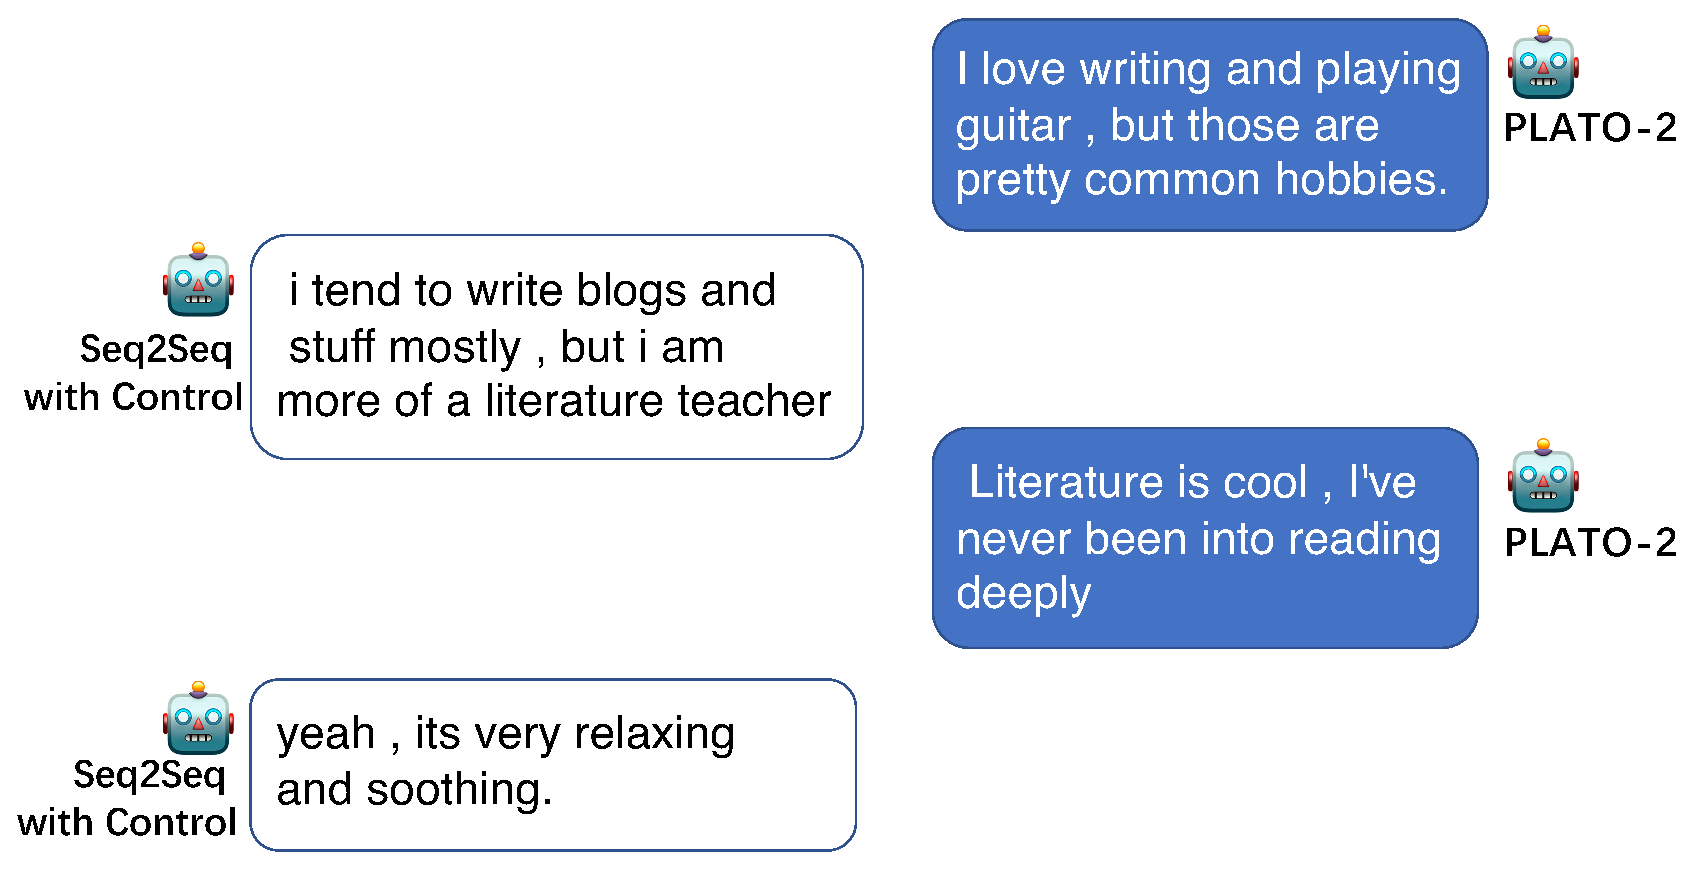
\includegraphics[width=\linewidth]{crop2.eps}  
  \caption{A small fragment of conversation between bot and bot% \KZ{crop the margins
%in this pic or use eps for both.} 
}
  \label{fig:sub-second}
\end{subfigure}
\caption{Small fragments from the chat logs between humans-bot and bot-bot}
\label{fig:two convs}
\end{figure}

Our framework consists of two components: \textit{competition} and 
\textit{scoring}, which may happen simultaneously. The competition is modeled
after most sport tournaments such as soccer or ping pong. 
There are three levels of competitions: 
game-level, match-level and tournament-level. 
Each match consists of several games. During a game, two bots will converse 
freely with each other and a virtual judge will score their performances according to
a group of criteria such as consistency and fluency, etc. 
%As an example like \figref{fig:example} shows, 
%Bot $A$ will be 
%penalized twice for repeating while Bot $B$ will be penalized once for 
%contradicting itself. In addition to the penalty, 
%a bonus point is rewarded to $A$
%who shows to produce relevant response with long term memory. 
%\KZ{Do we still have this as a criterion?}
%However, the specific bonus and penalty settings may vary 
%depending on the domain and scenarios that the experiment is 
%set in. 

%\begin{figure}[th!]
%	\centering
%	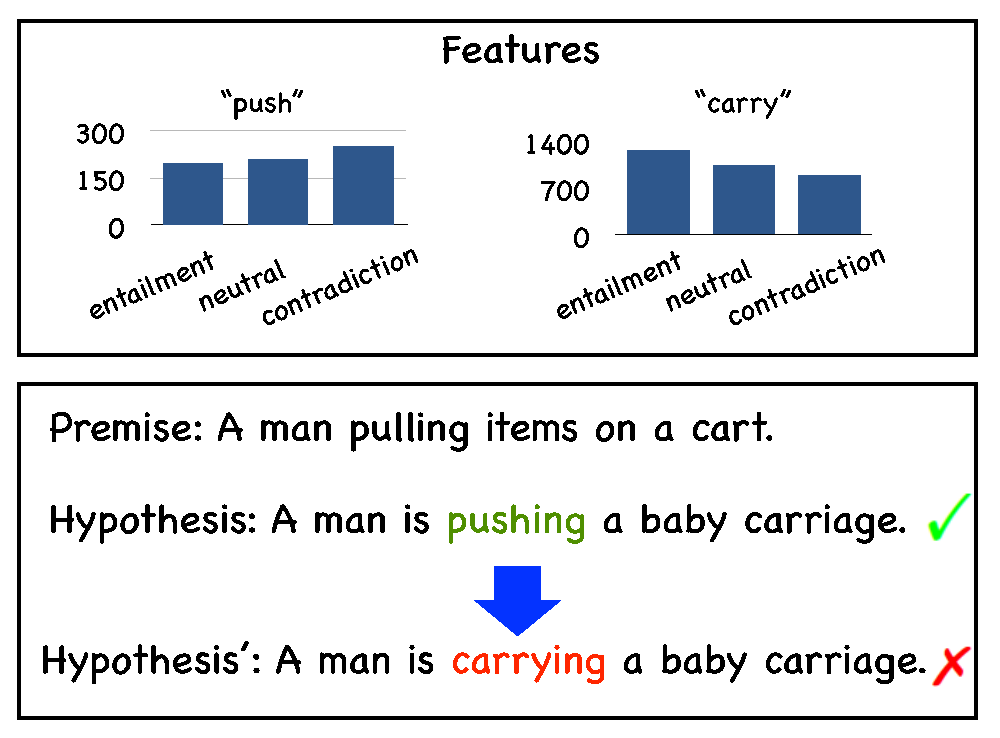
\includegraphics[width=0.95\columnwidth]{example.eps}
%	\caption{A chat snippet between two bots.}
%	\label{fig:example}
%\end{figure}

The main contributions of this paper are:
\begin{itemize}
\item We propose the first interactive evaluation framework for chatbots which
is based solely on bot-to-bot conversations and modeled after sports competitions (\secref{sec:competition}).
\item  The entire scoring process is fully automated and efficient. 
The system can rank seven bots in three minutes on average.
(\secref{sec:scoring}, \secref{sec:time}).
\item  Our experiments show that our scoring system closely tracks the 
human evaluation results. Preliminary results also show
that our evaluation system outperforms 
several recent strong baseline evaluation systems (\secref{sec:main}).
\item %We demonstrate the improvements in efficiency 
%using direct chat logs between bots.
We show that the chats between bots are impressively informative, 
even richer than the chats between humans and bots.
This suggests some possible directions to improve 
the capabilities of bots in the future.
(e.g., by having them learn from each other)  (\secref{sec:diversity})
\end{itemize}

\section{Problem Definition}
\label{sec:problem}

In this section we formally define the problem of short title extraction.
A char is a single Chinese or English character.
A segmented word (or term) $x$ is a sequence of several chars such as 
``Nike'' or ``牛仔裤''(jean).
A product title, denoted as $X$, is a sequence of words $\{x_1, x_2, ..., x_n\}$.
Let $Y$ be a sequence of labels $\{y_1, y_2, ..., y_n\}$ over $X$, where $y_i \in \{0, 1\}$.
The corresponding short title is a subsequence of $X$, denoted as $S = \{x_i\}$, 
where $y_i = 1$ and $|S| \le n$.

%we are interesting in obtaining a short title which can represent the most important information about the product.

We regard short title extraction task as a sequence classification problem.
Each word is sequentially visited in the original product title order
and a binary decision is made.
We do this by scoring each word $x_i$ within $X$ and predicting a label $y_i \in \{0, 1\}$, 
indicating whether the word should or should not be included in the short title $S$.
As we apply supervised training, the objective is to maximize the likelihood of all word labels
$Y=\{y_1,y_2,...,y_n\}$, given the input product title $X$ and model parameters $\theta$:
\begin{equation}
\label{eqn:problem}
\log{p(Y|X,\theta)}=\sum_{i=1}^{n}{\log{p(y_i|X,\theta)}}.
\end{equation}

%Our problem is different from Sequece Labelling problem, as ...

%In a more restrictive scenario, the number of words $m$ in the short title is strictly limited, where $m$ is some fixed number and $m \le \sum_{i=1}^{n} len(x_i)$. $len(x_i)$ is the number of words (chars) in term $x_i$.


\chapter{Methods}

In the previous section we talked about the background and demand for sentiment analysis system, the history of research, the general goal and challenges in this area, and some specific tasks for the researchers to work on. In this section, we will introduce some methods used for solving some of the tasks defined above; specifically, we will put most of our attention to statistical and machine learning methods, because of their generalization ability - one method can often be applied to many similar tasks with similar formulations without us having to look at the data and hand-craft features.

We will start with some important features; then we will talk about topic modeling methods that are widely used in factual information analysis, and their variations designed specifically for sentiment analysis problems; finally we will talk about the deep learning methods for natural language processing. In the past several years, we witnessed the ``tsunami" of deep learning in many fields, especially in computer vision and speech recognition. We will briefly introduce the history of deep learning, with an emphasis of its application in natural language processing, and then introduce several important models including word embedding, neural network language model and recurrent neural network, which are used in our framework.

\section{Features}

In the data-driven approaches for natural language processing, we often convert a piece of text into a feature vector that the statistical models can process. A large volume of work is devoted to the feature selection problem of machine learning. However, the discussion of such techniques is out of the scope of this paper. Instead, we will focus on some important features and related methods specific to sentiment analysis.

\subsection{Term Presense and Frequency}

In information retrieval, it is traditional to represent a text as a feature vector where each entry of the vector corresponds to the number of appearances of some specific term in the text. This frequency-based fashion is popular in information retrieval, seen in examples like the widely used tf-idf weighting. However, it is reported in \cite{pang2002thumbs} that in polarity classification, a better performance can be obtained using presence instead of frequency. Using presence means that each entry of the feature vector merely indicates whether a term appeared or not in the text. This observation shed light on the difference of topic-based and sentiment-based problems: while a topic is more likely to be emphsized by the frequent appearances of certain words, sentiment might not be strengthened by such repetition. 

One natural extention to single term frequency is higher-order n-grams. The effectiveness of using n-grams is yet to be discussed. \cite{pang2002thumbs} reported that higher performance can be achieved with unigrams than bigrams when classifying movie reviews by sentiment polarity, whilc \cite{dave2003mining} reported that in some settings bigrams can trigrams can outperfom unigrams in product review polarity classification.

\subsection{Part-of-speech}

One of the reasons that part-of-speech information's wide use in not just sentiment analysis but general text analysis is: part-of-speech tagging is a crude form of word sense disambiguation. One of the earliest use of data-driven approach for the prediction of semantic orientation of words was developed for adjectives. Subsequent work on subjectivity detection demonstrated a high correlation between the use of adjectives and subjectivity \cite{hatzivassiloglou2000effects}. This observation has often been seen as an evidence that certain adjectives are good indicators of sentiment. In extention to just using adjectives, \cite{turney2002thumbs} proposed to use a number of pre-defined part-of-speech pattern to select phrases (most contain adjectives or adverbs), which is later used to detect document sentiment. Beside adjectives, verbs and nouns can also be used for expressing sentiment; as reported in \cite{pang2002thumbs}, using only adjectives as features lead to much worse performance than using the same number of most frequent unigrams. 
% For sentiment analysis, adjectives have been used as important features in a number of works \cite{mullen2004sentiment,whitelaw2005using}. 

\subsection{Negations}

Negations is a key factor in the expression of sentiment, because a single negation can completely reverse the sentiment polarity. Despite of the semantic importance, negations are not specifically treated in term-based vector representations. This is not much of a problem in information retrieval since a negation cannot drastically change the topic of a piece of text. However, this is problematic for sentiment analysis, especially when there is double negation. It is possible to deal with negations indirectly using second-order features, that is, for example \cite{das2001yahoo} proposed to attach ``NOT" to words occuring close to negation terms. This can be extended to a more subtle and accurate method by using at the parsing tree. In \cite{na2004effectiveness}, the authors looked for specific part-of-speech tag patterns for negations, and tag the complete phrase as a negation phrase. Further improvement is achieved by using deeper analysis of the syntax \cite{kennedy2006sentiment}.

\section{Topic Modeling Methods}

Topic modeling is a method for analyzing large quantities of unlabeled data - it's an unsupervised method. For the purpose of sentiment analysis, or more generally text analysis, a topic is a probability distribution over a collection of words. A topic model is generative model that describes the procedure of the generation of the topics, defined by the statistical relationship between a group of observed and latent random variables. The goal of having the topics is to provide a thematic summary of a collection of documents - they tell us about the themes of those documents. For example a collection of news articles might have themes of politics, business, culture, and science.

\subsection{Latent Dirichlet Allocation}

Latent Dirichlet Allocation (LDA) \cite{blei2003latent} is arguably the most popular topic model in application; it is also very simple. At a high level viewpoint, LDA provides a model that describes the generation process of each document in a collection. The collection of documents is denoted as $D$, and the vocabulary set is denoted as $V$. LDA requires a constant $K$ - the number of topics, it needs to be defined beforehand.
Each topic $i$ of LDA is model by a multinomial distribution $\beta_i$ of all the  words in $V$. Each document is modeled as a multinomial distribution $\alpha$ over the $K$ topics. The generation process is:

For each document:
\begin{itemize}
    \item[1.] draw a topic distribution over the $K$ topics, $\theta\sim \text{Dir}(\alpha)$; $\text{Dir}(\alpha)$ is the dirichlet distribution with scaling factor $\alpha$; $\theta$ is a vector of length $K$ denoting the probability of each topic;
    \item[2.] for each word $w_n$ in the document:
        \begin{itemize}
            \item[i.] draw a topic $z_n\sim \text{Mult}(\theta)$ from the $K$ topics; $\text{Mult}(\theta)$ is a multinomial distribution defined by $\theta$;
            \item[ii.] draw a word $w_n\sim \beta_{z_n}$.
        \end{itemize}
\end{itemize}

Note that $\alpha$ is actually $(\alpha_1, \alpha_2, ..., \alpha_K)$, $K$ parameters for the dirichlet distribution.
We use a one-hot vector $w$ to represent a word, and if the integer index of thw word in the dictionary is $u$, then $w^u=1$ and $w^v=0$ for all $v\neq u$. We use $\vw=(w_1, w_2, ..., w_N)$ to denote a document with $N$ words.
We use a one-hot vector $z$ to represent the selection of topic - the $i$th element of $z$ is 1 if we select the $i$th topic. We use $\vz=(v_1, v_2, ..., v_N)$ to represent the topic selction of the whole document. $\beta$ is a $K\times V$ word-probability matrix for each topic (row) and each word (column), $\beta_{i,j} = p(w^j=1|z^i=1)$

Before diving into the inferential problem of LDA, we emphasize on several characteristics of the LDA model:

\begin{itemize}
    \item the documents in collection $D$ share the same set of topics;
    \item from process 1. we see that LDA allows each document can contain multiple topics
    \item from process 2. we see that LDA treats each document as a bag of words - the order of the words is ignored;
    \item in LDA, each word is generated from a single topic
    \item topics are allowed to shift quickly - the topic of each word is sampled independently of other words.
\end{itemize}

The inferential problem of LDA is determining the posterior distribution of the latent variables given the observed variables - the documents:

$$p(\theta, \vz | \vw, \alpha, \beta) = \frac{p(\theta, \vz, \vw | \alpha, \beta)}{p(\vw | \alpha, \beta)}$$

We can decompose the numerator into a hierarchy by examing the graphical model:
$$p(\theta, \vz, \vw | \alpha, \beta) = p(\vw | \vz, \beta)p(\vz | \theta)p(\theta| \alpha)$$
As LDA treats the document as a bag of word, $p(\vw | \vz, \beta) = \prod_{n=1}^N \beta_{z_n, w_n}$. Also $p(\vz | \theta)$ is trivial and we can write $p(z_n | \theta)=\theta_i$ such that $z_n^i=1$. Finally, $p(\theta | \alpha)$ is given by:

$$p(\theta | \alpha) = \frac{\Gamma(\sum_{i=1}^K \alpha_i)}{\prod_{i=1}^K \Gamma(\alpha_i)} \prod_{i=1}^K \theta_i ^ {\alpha_i - 1}$$

Putting all these together we have the numerator:

$$p(\theta, \vz, \vw | \alpha, \beta) = \left(\frac{\Gamma(\sum_{i=1}^K \alpha_i)}{\prod_{i=1}^K \Gamma(\alpha_i)} \prod_{i=1}^K \theta_i ^ {\alpha_i - 1}\right) 
\prod_{n=1}^N \prod_{i=1}^K \prod_{j=1}^V (\theta_i \beta_{i,j})^{w_n^jz_n^j}$$

To obtain the denominator, we marginalize over $\theta$ and $\vz$:

$$p(\vw | \alpha, \beta) = \frac{\Gamma(\prod_{i=1}^K \alpha_i)}{\prod_{i=1}^K \Gamma(\alpha_i)} \int \left(\prod_{i=1}^K \theta_i^{\alpha_i - 1}\right)
\left(\prod_{n=1}^N \sum_{i=1}^K \prod_{j=1}^V (\theta_i\beta_{i,j})^{w_n^j}\right)
d\theta $$

Computing this distribution is intractable as the coupling between $\theta$ and $\beta$ makes it so that when we compute the log of this function, we are unable to seperate the $\theta$ and $\beta$. While the exact inference is intractable, various approximate inference techniques can be used, including Gibbs sampling and variational inference. However the introduction of inference methods is out of the scope of this paper since we want to focus on the models, so we will not skip it and encourage the readers to refer to \cite{steyvers2005probabilistic,blei2012probabilistic} for more details. 

To use LDA for text analysis, we need to provide a set of documents and the number of topics $K$. LDA will give us two kinds of distributions: $K$ topics shared across the whole collection, each being a distribution over the whole dictionary; for each document a distribution of the topics. 

\subsection{Variations of LDA}

LDA models a simple generation process which fits many scenarios. However, when used for the extraction of aspects for aspect-based sentiment analysis, due to the problem characteristics analyzed in Chapter 2, the performance of LDA is not satisfactory. Many varaitions of LDA have been proposed specifically for sentiment analysis.

Since in evaluative texts like product reviews, there are aspect words and sentiment words, one design factor of topic model is to use one latent variable for both types or to use seperate latent variables. In addition, the model can also be enhanced by modeling the dependency between aspects and ratings. One can also choose to model only the opinion phrases instead of all the words in the document. Here we first review the formal definition of the graphical model of LDA, as shown in Figure~\ref{fig:methods:LDA_1}:

$$p(\vz, \vw, \theta | \alpha, \beta) = p(\theta, \alpha) \prod_{n=1}^N \left[ 
p(z_n| \theta) p(w_n | z_n, \beta)\right]$$

\begin{figure}
\centering
\includegraphics[width=0.5\columnwidth]{figures/methods/LDA_1}
\caption{LDA graphical model. Source of figure: \cite{moghaddam2012design}.}
\label{fig:methods:LDA_1}
\end{figure}

\subsubsection{S-LDA: seperate aspect and rating}

In S-LDA \cite{lakkaraju2011exploiting,moghaddam2012design}, the latent variable for topics $\vz$ is replaced by two seperate variable for aspects and rating respectively. For each aspect-rating pair, $\theta$ contains the probability of generating the corresponding combination. For each review, $\theta$ is sampled once, just like LDA; then $a_n$ and $r_n$ are sampled independently for each word and $w_n$ is sampled conditioned on both latent variable. The formal definition of the generation process is the following, as shown in Figure~\ref{fig:methods:S-LDA}:

$$p(\va, \vr, \vw, \theta | \alpha, \beta) = p(\theta, \alpha) \prod_{n=1}^N \left[ 
p(a_n| \theta) p(r_n | \theta) p(w_n | a_n, r_n, \beta)\right]$$

\begin{figure}
\centering
\includegraphics[width=0.5\columnwidth]{figures/methods/S-LDA}
\caption{S-LDA. \cite{moghaddam2012design}}
\label{fig:methods:S-LDA}
\end{figure}

\subsubsection{D-LDA: dependency between aspect and rating}

Several variations of LDA leveraged the dependency between aspects and ratings \cite{he2011automatically,jo2011aspect,li2010sentiment,lin2009joint,moghaddam2011ILDA,moghaddam2012design}.
On the basis of S-LDA, D-LDA further models the dependency of the rating on the aspect. The generation process is the following, as shown in Figure~\ref{fig:methods:D-LDA}:

$$p(\va, \vr, \vw, \theta | \alpha, \beta) = p(\theta, \alpha) \prod_{n=1}^N \left[ 
p(a_n| \theta) p(r_n | a_n, \theta) p(w_n | a_n, r_n, \beta)\right]$$

\begin{figure}
\centering
\includegraphics[width=0.5\columnwidth]{figures/methods/D-LDA}
\caption{D-LDA. \cite{moghaddam2012design}}
\label{fig:methods:D-LDA}
\end{figure}

\subsubsection{PLDA: model only opinion phrases}

While LDA assumes that a document is a bag of words, P-LDA \cite{zhan2011semantic,moghaddam2012design} assumes that a document is a bag of opinion phrases. A document is preprocessed to contain only opinion phrases, each being a head-modifier pair $<h_n, m_n>$. Thus, instead of one, the observed variable in P-LDA is two - a head and a modifier, resulting in the generation process as shown in Figure~\ref{fig:methods:P-LDA}:

$$p(\vz, \vh, \vm, \theta | \alpha, \beta, \pi) = p(\theta, \alpha) \prod_{n=1}^N \left[ 
p(z_n| \theta) p(h_n, m_n | z_n, \beta, \pi)\right]$$

\begin{figure}
\centering
\includegraphics[width=0.5\columnwidth]{figures/methods/P-LDA}
\caption{P-LDA. \cite{moghaddam2012design}}
\label{fig:methods:P-LDA}
\end{figure}

\subsubsection{S-PLDA}

Combining S-LDA and PLDA, we have S-PLDA \cite{moghaddam2012design} as shown in Figure~\ref{fig:methods:S-PLDA}:

$$p(\va, \vr, \vh, \vm, \theta | \alpha, \beta, \pi) = p(\theta, \alpha) \prod_{n=1}^N \left[ 
p(a_n| \theta) p(r_n | \theta) p(h_n | a_n, \beta) p(m_n | r_n, \pi)\right]$$

\begin{figure}
\centering
\includegraphics[width=0.5\columnwidth]{figures/methods/S-PLDA}
\caption{S-PLDA. \cite{moghaddam2012design}}
\label{fig:methods:S-PLDA}
\end{figure}

\subsubsection{D-PLDA}

By adding the aspect-rating dependency to S-PLDA, we have D-PLDA \cite{moghaddam2011ILDA,moghaddam2012design}, as shown in Figure~\ref{fig:methods:D-PLDA}:

$$p(\va, \vr, \vh, \vm \theta | \alpha, \beta, \pi) = p(\theta, \alpha) \prod_{n=1}^N \left[ 
p(a_n| \theta) p(r_n | a_n, \theta) p(h_n | a_n, \beta) p(m_n | a_n, r_n, \pi)\right]$$

\begin{figure}
\centering
\includegraphics[width=0.5\columnwidth]{figures/methods/D-PLDA}
\caption{D-PLDA. \cite{moghaddam2012design}}
\label{fig:methods:D-PLDA}
\end{figure}

\subsubsection{MG-LDA}

Since aspect extration is a multi-document summarization, the dataset we use is a set of reviews about different products. For example when we perform aspect extraction for hotels, we might use user reviews for different hotel in various cities. Thus in the reviews there are topics that are specific to some particular hotel or a subset of hotels, for example \emph{hotels in Paris}, \emph{youth hostels}. They are valid topics, however not appropriate for ratable aspects. These topics are correlated with the specific product, hence is shared across the scope of the whole review; the topics that can be used as aspects, as analyzed in the previous chapter, are often talked about in segments of the review. The features specific to some product might be prominent at the scope of one review, but if we break down the reivews into sentences, the occurrance of such features specific will be ``diluted" and the aspect topics are more prominent. Motivated by this observation, the authors of MG-LDA \cite{titov2008modeling} introduced two kinds of topics: \emph{local topics} are the ones observed locally in several consecutive sentences, and are appropriate as aspects; \emph{global topics} are the ones closely related to the product and shared across a single review. The generation of words is thus different from that of LDA: now we use a combination of two topic distribution, one global topic that determines the features specific to the product we review, and a local topic that determines which aspect of the product we will talk about. The structure of MG-LDA is shown in Figure~\ref{fig:methods:MG-LDA}. For each document, the global topic distribution is sampled once, since only target product is consistent throughout the review; the local topic distribution is sampled for each sliding window, thus is sampled multiple times across the review, representing the aspect shifting from window to window; each word in a single window is generated by sampling from both topic distributions and combining them.
\begin{figure}
\centering
\includegraphics[width=0.5\columnwidth]{figures/methods/MG-LDA}
\caption{MG-LDA. Source of figure: \cite{titov2008modeling}.}
\label{fig:methods:MG-LDA}
\end{figure}

MG-LDA was designed specifically for aspect extraction, without distinguishing aspects and sentiments. MG-LDA has been shown to perform better than other LDA variations mentioned above, so we will make a direct comparison with our model  in our experiment chapter.

\section{Deep Learning for Natural Language Processing}


\begin{displayquote}
 ``Deep Learning waves have lapped at the shores of computational linguistics for several years now, but 2015 seems like the year when the full force of the tsunami hit the major Natural Language Processing (NLP) conferences." - Dr. Christopher D. Manning, Dec 2015 
\end{displayquote}

Deep learning has drawn a lot of attentiono in recent years, and we have already seen many applications of it in natural language processing. In this section we will first give a brief introduction to the history of deep learning; then we will introduce several widely used deep learning methods for natural language processing. 

\subsection{A Brief History of Deep Learning}

The core model of deep learning is neural network. The earliest neural-network-like algorithms that had multiple layers of no-linear features can be traced back to \cite{ivakhnenko1965cybernetic}, where the authors used a thin but deep models with polynomial activation functions which they analyzed with statistical methods. In each layer, they select the best features through statistical methods and forward them to the next layer. They did not use backpropagation to train their network end-to-end but used layer-by-layer least squares fitting where previous layers were independently fitted from later layers.

The earlist convolutional network appeared in \cite{fukushima1979organization}. Their networks had multiple convolutional and pooling layers similar to modern networks, but the network was trained by using a reinforcement scheme where a tail of strong activationo oin multiple layers was increased over time.

Backpropagation of erros that are used to train deep models was lacking at this point. It was derived already in the early 1960s but in an inefficient and incomplete form. The modern form was derived first by Linnainmaa in his 1970 masters thesis, however he did not mention its application to neural networks. Even at this point, backpropagation was relatively unknown and very few documented applications of backpropagation in the early 1980s. \cite{rumelhart1988learning} showed that backpropagation used for neural networks could yield interesting distributed representations. At this time, this was an important result in cognitive psychology where the questiono was whether human cognition can be thought of as relying on distributed representations (connectionism) or symbolic logic (computationalism).

The first practical application of backpropagation cam about through \cite{lecun1989backpropagation} where the authors used convolutional networksin combination with backpropagation to classify handwritten digits (MNIST) and this system was later used to read large numbers of handwritten checks in the United States. Despite these successes, funding for research into neural networks was scarce. The term artificial intelligence dropped to near pseudoscience status during the ``AI winter". Some important advances were made in this time, for example, long short-term memory (LSTM) for recurrent neural network \cite{hochreiter1997long}, but these advances went mostly unnoticed util later as they were overshadowed by support vector machine (SVM) \cite{cortes1995support}.

The next big shift occured just by waiting for the computers to get fater, and then later by the introduction of GPU. In this period, neural networks slowly began to rival SVMs. The main difficulty at this point was to train big, deep networks, which suffered from vanishing gradient problem, where features in early layers could not be learned because no learning signal reached these layers.

The first solution to this problem was layer-by-layer pre-training, where the model is built in a layer-by-layer fashion by using unsupervised learning method. The first pre-training approaches was proposed for recurrent neural networks by \cite{schmidhuber1992learning}, and then for feed-forward networks by \cite{hinton2006reducing}, which started the fever of neural networks.

\subsection{Word2Vec}

As natural language processing often treats words as the basic unit of study and neural networks takes vectors as input, it is natural to represent words by vectors. The most basic model is one-hot vector, where each vector has the size of the vocabulary, and one non-zero entry denoting the word. This simple design has several drawbacks: first it's dimensionality is too large if we have a large dictionary; secondly and more importantly, the vector representation does not capture any semantic information of the words. To improve the vector representation of words, we replace the original high-dimensional discrete vector with a lower-dimensional real-valued vector; instead of the pre-defined fixed values, we train the vector representations so that the cosine similarity of two word vectors captures the semantic similarity of the two corresponding words. This Word2Vec \cite{mikolov2013distributed} model adopted a heuristic: if two words often appear close to each other, then they are similar, and this is called word embedding - embed a word's meaning in the the words surrounding it. Also, the semantics of each word is stored in all the entries of the word vector, so the word vector we learned is called a \emph{distributed representation}.

Word2Vec contains two seperate models: skip-gram and CBOW. The two models can used independently two train two vectors for each word, and concatenate the two vectors to obtain the final word embedding. However in practice, people often use only the skip-gram model with special training techniques like negative samping and noise contrastive estimation. In our paper, we introduce skip-gram with negative sampling.

For a high level interpretation, we consider a single word $w$ in a sentence: skip-gram asks us to predict each other word, or context word $c$, in the sentence with $w$; this way we embed the meaning of the context in the representation of $w$. For a more formal definition, we consider all the word-context pairs $(w,c)$ in a corpus $D$, and we consider the conditional probabilities $p(c|w)$. We use $C(w)$ to denote the set of contexts of word $w$, and $\theta$ as the parameters of $p(c|w; \theta)$. Our goal is to find the parameters that maximize the corpus probability.

$$\theta = \argmax_{\theta} \prod_{w\in W} \left[\prod_{c\in C(w)} p(c|w; \theta) \right]\text{;  or alternatively}$$
$$\theta = \argmax_{\theta} \prod_{(w,c)\in D} p(c|w; \theta)$$

When predicting each context word $c$ with word $w$, the model uses a softmax:

$$p(c|w;\theta) = \frac{e^{v_c\cdot v_w}}{\sum_{c'\in C}e^{v_{c'}\cdot v_w}}$$

where $v_c, v_w, v_{c'} \in \mathbb{R}^d$ are vector representations of $c, w, c'$ respectively; $C$ is the set of all available contexts. Maximizing the above conditional probability is equivalent to maximizing the objective:

$$\argmax_{\theta}\sum_{(w,c)\in D} \log p(c|w)
= \sum_{(w,c)\in D} (\log e^{v_c\cdot v_w} - \log\sum_{c'\in C}e^{v_{c'}\cdot v_w})$$

While the above objective can be computed, but it's computationally expensive to do so, because the summation will iterate over all the contexts $c'$. One way of making the computation more tractable is to replace the summation with a sampling of random noises, this is called negative sampling. Note that other methods like noise contrastive estimation \cite{mnih2013learning} and importance sampling \cite{bengio2003quick,bengio2008adaptive} all share the same basic idea, and we will not elaborate on thess two other models in this paper.

With negative sampling, the model is actually optimizing a different objective. Consider a word-context pair $(w,c)$, we denote by $p(D=1|w,c)$ the probability that $(w,c)$ came from the corpus, correspondingly, $p(D=0|w,c)=1-p(D=1|w,c)$ denotes the probability did not come from the corpus. Still with parameters $\theta$, our goal is now to maximize the probabilities that all the observed pairs indeed came from the corpus:

\begin{align*}
    &\argmax_{\theta}\prod_{(w,c)\in D} p(D=1|w,c;\theta) \\
    &=\argmax_{\theta} log \prod_{(w,c)\in D} p(D=1|w,c;\theta) \\
    &=\argmax_{\theta} \sum_{(w,c)\in D} \log p(D=1|w,c;\theta)
\end{align*}

The conditional probability $p(D|w,c|\theta)$ is defined using softmax:

$$p(D=1|w,c;\theta)=\frac{1}{1+e^{-v_c\cdot v_w}}$$

leading to the objective:

$$\argmax_{\theta}\sum_{(w,c)\in D}\log \frac{1}{1+e^{-v_c\cdot v_w}}$$

This objective has a trivial solution if we set $\theta$ so that $v_c=v_w$ and $p(D=1|w,c;\theta)=1$ all the time. But we of course don't want all the words share a same representation and we will disallow some $(w,c)$ pairs. One way to do so is to make $p(D=1|w,c;\theta)$ low for some pairs, i.e. pairs not observed in the data. This is achieved by generating the set $D'$ of random $(w,c)$ pairs and assuming they are out of the corpus - hence ``negative samples". Let $\sigma(x)=\frac{1}{1+e^{-x}}$, the new objective is:

\begin{align*}
    &\argmax_{\theta}\prod_{(w,c)\in D} p(D=1|w,c;\theta) \prod_{(w,c)\in D'}p(D=0|w,c;\theta) \\
    =&\argmax_{\theta}\prod_{(w,c)\in D} p(D=1|w,c;\theta) \prod_{(w,c)\in D'}(1-p(D=1|w,c;\theta)) \\
    =&\argmax_{\theta}\sum_{(w,c)\in D} \log p(D=1|w,c;\theta) + \sum_{(w,c)\in D'} \log(1-p(D=1|w,c;\theta)) \\
    =&\argmax_{\theta}\sum_{(w,c)\in D} \log\sigma(v_c\cdot v_w) + \sum_{(w,c)\in D'} \log\sigma(-v_c\cdot v_w)
\end{align*}

This model can then be trained end-to-end much more efficiently and the final parameters $\theta$ contains all the word vectors. This objective has been shown to be equivalent to factorizting a shifted PMI matrix \cite{levy2014neural}, which means that the semantic similarity captured by Word2Vec is actually the point-wise mutual information between the pair of words. Their are other models of vector representation for words, including \cite{pennington2014glove,shazeer2016swivel}, but Word2Vec is by far the most widely used word vector in applications.


\subsection{Neural Network Language Model}

The goal of statistical language model is to learn the joint probability function of sequences of words in a language. This is difficult due to the curse of dimensionality: there are too many possible sequences. Traditional approaches based on n-grams obtain generalization ability by concatenating very short overlapping sequences, focusing on only a local window each time. In neural network language models, the index-based word representation used in traditional n-gram models is replaced with distributed representations like Word2Vec. This allows the model to be informed about an exponential number of semantically neighboring words each time, due to the semantic embedding in each word vector. With word vectors, the model simultaneously learns the representation of each word and the probability function of the sequence. The generalization ability is improved because each word now shares its information with many other similar words, replacing a word in a already seen sequence with a semantically similar word will now result in a similar probability function.

A statistical language model can be defined by the conditional probability of the next word given previous words: $p(w_1^T) = \prod_{t=1}^T p(w_t | w_1^{t-1})$. The earliest neural network language model was proposed in \cite{bengio2000a} and follows the n-gram approach, which means that it approximate the conditional probability:

$$p(w_t | w_1^{t-1}) \approx p(w_t | w_{t-n+1}^{t-1})$$

The modeling of function $f(w_t,..., w_{t-n+1}) = p(w_t | w_1^{t-1})$ is done by two steps:

\begin{itemize}
    \item[1.] By using a matrix $C$ of shape $|V|\times m$, where $V$ is the vocabulary and $m$ is the dimension of word vector, we map the input sequence $(w_{t-n+1}, ..., w_{t-1})$ to a sequence of word vectors $(C(w_{t-n+1}), ..., C(w_{t-1}))$;
    \item[2.] A function $g$ maps the input sequence of word vectors to a conditional probability distribution over all the words in $V$ for the next word $w_t$. The output is a probability vector whose $i$th element estimates $p(w_t=i|w_1^{t-1})$.
\end{itemize}
$$f(i, w_{t-1}, ..., w_{t-n+1}) = g(i, C(w_{t-1}), ..., C(w_{t-n+1}))$$

Note that among the two mappings $g$ and $C$, the later is shared across all the words in the context, holding all the $|V|$ word vectors in rows. Function $g$ is designed to be a feed-forward neural network with parameters $\omega$, so the whole parameter set is $\theta={C, \omega}$. The objective is to minimize the log-likelihood of the entire corpus ($T$ word sequences):

$$L=\frac{1}{T} \sum_t \log f(w_t, w_{t-1}, ..., w_{t-n+1}; \theta) + R(\theta)$$

where $R(\theta)$ is a regularization term designed for avoiding over-fitting of the neural network. 

The input layer of the network receives the sequence of words, map them into a sequence of word vectors and pass it to a normal tangent hidden layer and obtain the outputs $y_i$ for word $i$. The output layer, similar to what is used in skip-gram in Word2Vec, is a softmax output layer:

$$p(w_t | w_{t-1}, ..., w_{t-n+1}) = \frac{e^{y_{w_t}}}{\sum_i e^{y_i}}$$

where $y$ is given by the hidden layer computation:

$$y=b+Wx+U\tanh(d+Hx)$$

where the hyperbolic tangent is applied element-wise; $x$ is the concatenation of the input word vectors:

$$x=(C(w_{t-1}), C(w_{t-2}), ..., C(w_{t-n+1}))$$

The whole model is then trained end-to-end, simultaneously learning the representation of words and the probability function for sequences.

The model has several restrictions to this language model that is based on a feed-forward neural network. First the computational cost at the softmax layer is very high, similar to what we see from Word2Vec, but this time we cannot directly use negative sampling, because we need to consider the $n-1$ previous words, instead of only one word. Importance sampling can be applied to this scenario with some careful modification \cite{cho2015on}. Another way to solve this problem is to replace the flat softmax with some hierarchical structure, that is, using a hierarchical softmax \cite{mikolov2013efficient}. Also the normalization of the softmax can be replaced by a self-normalizing term learned jointly with the model \cite{devlin2014fast}. Beside the computational efficiency, this model is restricted to using local features - only previous $n-1$ words are used for predicting the next word. To address this problem, we adopt recurrent neural network, which is specifically designed for modeling sequences of different lengths.

\subsection{Recurrent Neural Network}

The idea behind recurrent neural network (RNN) is to make use of sequential information. In traditional layer structured neural network, we assume that all inputs (and outputs) are independent of each other. But for tasks like language modeling this is a huge restriction. RNN is ``recurrent" because it performs the same process for every element in a sequence, with the output being depended on the previous computations. Another way to think about RNN is that it has a ``memory" which captures imformation about what has been calculated so far. In theory RNN can make use of information in arbitrarily long seuqnces, but inpractive they are limited to looking back only a few steps.

The computation of RNN is slightly different from normal neural network which is a stack of layers, instead of going through the fixed structure of layers, RNN carry out its computation in multiple time steps. The time steps of RNN actually correspond to the layers of normal neural network, however the depth of layers is not pre-defined and varys according to the input sequence. RNN has two core functions which it performs at each time step: update of its internal state, and output based on its internal state; the later is optional.

The abstraction of RNN internal state update is simple: $h_t=\RNN(h_{t-1}, x_t)$, where $h_t$ is the new state, $h_{t-1}$ is the previous state, $x_i$ is the input at this time step, all of them are vectors; $\RNN$ encapsules the computation of an RNN layer, which in the most simple form is just linear transformations followed by a non-linearity (biases are dropped for simplicity):

$$RNN(h_{t-1}, x_t) = tanh(Wh_{t-1} + Ux_t)$$

The output part of RNN is also simple. Let us consider the scenario of language modeling. At each time step $t$ we have a hidden state $h_t$ which contains the information of all previous words $(x_1, ..., x_t)$. With this state we can predict the next word $x_{t+1}$ by computing a softmax over all possible words, which gives us the probability of next word $x_{t+1}$ conditioned on the previous words, therefore we can model the probability of the whole sequence with this RNN. After training the RNN for language modeling, it can be further used for generating sequences: at each time, take the word with the highest probability predicted by the softmax; then feed the predicted output to the RNN as an input; proceed until the RNN outputs a special symbol denoting the end of the sequence.

\begin{figure}
\centering
\includegraphics[width=0.7\columnwidth]{figures/methods/RNN}
\caption{The rolled and unrolled forms of RNN. Source: \emph{Nature}.}
\label{fig:methods:RNN}
\end{figure}

The rolled and unrolled forms of RNN is shown in Figure~\ref{fig:methods:RNN}. It is important to remember that almost all RNN structures follow the abstraction above, though the instantiation of the $\RNN$ function might be much more complicated. With this abstraction, we can see the correspondence between RNN and a traditional neural network structure: the hidden states of RNN correspond to the activations of a normal NN's hidden layers, but the parameters are shared across layers. This correspondence leads us to the training algorithm for RNN - backpropagation through time (BPTT). After unrolling the RNN computation into layers similar to normal NN, we do backpropagation just like normal; but after updating the weights at all the layers - which are actually copies of a single layer, we take the average of those copies and use it as the new RNN layer.

Since RNN and normal NN use virtually the same training algorithm, the difficulty of training a deep neural network also occurs to RNN when the input sequence is long and the depth of RNN is correspondingly large. The main problem is the vanishing gradient problem \cite{hochreiter1991untersuchungen,hochreiter2001gradient}. The intuitive explaination of vanishing gradient is: RNN updates involves repeatedly multiplying a matrix to itself, and when the matrix entries are small, almost no gradient is passed to earlier layers. The result is: information learned at later time steps cannot be efficiently passed to earlier time steps, making it hard for RNN to learn long-distance dependencies in the sequence. Detailed analysis of the vanishing gradient problem can be found in \cite{pascanu2013on}. This problem makes RNN less useful for something like language modeling, which often involves long input sequences.

\subsubsection{Long Short-Term Memory}

Long Short-Term Memory \cite{hochreiter1997long} is a variation of RNN that is designed to address the vanishing gradient problem. The abstraction of LSTM is still the same to the original one: $h_i=\RNN(h_{t-1}, x_t)$; however the update function $\RNN$ is more complicated. LSTM introduced four new elements: input gate $i$, forget gate $f$, output gate $o$, and cell $c$; the formal update function is:

\begin{align*}
& i_t = \sigma(W^i x_t + U^i h_{t-1}) \\
& f_t = \sigma(W^f x_t + U^f h_{t-1}) \\
& o_t = \sigma(W^o x_t + U^o h_{t-1}) \\
& c_t = f_t \odot c_{t-1} + i_t \odot \tanh(Wx_t + Uh_{t-1}) \\
& h_t = o_t \odot \tanh(c_t)
\end{align*}

where $\sigma$ is the sigmoid function, $\odot$ denotes the element-wise product.

Despite the seemingly complicated design, there is a clear intuition behind LSTM. LSTM can be derived from normal RNN by two steps:

\begin{itemize}
    \item[1.] In the original RNN, the repeated multiplication introduced the vanishing gradient problem, so we replace the multiplications with additions. This is done by introducing the cell and update it with addition.
    \item[2.] There are three projections in RNN and we take care of them by using the three gates, so the model has the flexibility of deciding what informationo to pass to the next time step:
        \begin{itemize}
            \item input to hidden: input gate
            \item hidden to hidden: forget gate
            \item hidden to output: output gate
        \end{itemize}
    Now the cell keeps the real memory (hence the real ``hidden state"), and the hidden state is what the cell exposes to the next time step.
\end{itemize}

\begin{figure}
\centering
\includegraphics[width=0.7\columnwidth]{figures/methods/LSTM}
\caption{Long Short-term Memory. Source of figure: \cite{jozefowicz2015empirical}.}
\label{fig:methods:LSTM}
\end{figure}

The structure of LSTM is shown in Figure~\ref{fig:methods:LSTM}. The use of the gates is to allow the corresponding projection keep the original signal without applying any non-linearity, enabling part of the model to perform an identity mapping. Similar idea is recently applied to normal neural network by introducing ``residual connection", which is basically an identity mapping in addition to the original non-linear transformation. This significantly improved the performance of very deep neural netowrks (as deep as a thousand layers), related works can be found in \cite{srivastava2015highway, he2015deep, huang2016deep}.


\subsection{Paragraph Vector}
\label{section:paragraph_vector}
Using recurrent neural network is only one of the methods of sequence modeling. There are other methods which try to extend word2vec to phrase and sentence level. Given a vector representation of words, the most direct way of representing a sentence is taking the average of the corresponding word vectors. But this is obviously too simple, for the following reasons:

\begin{itemize}
    \item The words in a sentence should not be treated with equal attention. Different words are of different significance to the semantics of the sentence, hence in making the sentence representation, we should not use the same weight for all the words.
    \item The word order information is lost in this simple representation. Note that with the same set of words, different orders can render completely different meanings.
\end{itemize}

One way of making a better sentence representation is to leverage the parsing tree. In\cite{socher2011parsing}, the authors used a recursive neural network to process the parsing tree and build up the sentence representation along the tree structure. However this approach only works for sentences with good grammar because the final vector representation relies highly on the quality of the parsing tree.

In \cite{le2014distributed}, the authors proposed a much less complicated method which is a simple extension to the two models from word2vec, called paragraph vector. We will introduce the two extended models in the following.

\subsubsection{PV-DM}

\begin{figure}
\centering
\includegraphics[width=0.5\columnwidth]{figures/methods/PV-DM}
\caption{The distributed memory model for paragraph vector.}
\label{fig:methods:PV-DM}
\end{figure}

In the previous section, we introduced one of the two models in word2vec, skip-gram. In skip-gram, one single word is used to predict every other word in the sentence, so that through back-propagation, the semantics of all other words is embedded in the word representation, resulting in a semantic embedding. In PV-DM (distributed memory for paragraph vector), a similar idea is adopted - a single paragraph vector is used to predict every word in the paragraph, so it can capture the semantics of all the words. Concretely, the model is defined by the following network structure, as shown in Figure~\ref{fig:methods:PV-DM}:

\begin{itemize}
    \item Each word in the dictionary is mapped to a word vector which is shared across all the sentence, just like word2vec. We can use pre-trained word vectors and fix them when training the paragraph vectors, or we can train the two representations simultaneously.
    \item Each paragraph is mapped to a vector (not necessarily in the same space with the word vectors), which is then passed through a feed-forward neural network, followed by a softmax output layer, just like skip-gram.
    \item The network predicts each word in the paragraph, with an opitimization objective of the log-likelihood of the whole corpus.
\end{itemize}

The only difference from skip-gram is that the word vector used for prediction is replaced with a pargraph vector.

\subsubsection{PV-DBOW}

\begin{figure}
\centering
\includegraphics[width=0.5\columnwidth]{figures/methods/PV-DBOW}
\caption{The distributed bag-of-word model for paragraph vector.}
\label{fig:methods:PV-DBOW}
\end{figure}

PV-DBOW, or distributed bag-of-word for paragraph vector, is an extension to CBOW, continuous bag-of-word from word2vec. CBOW is defined by a n-gram neural network language model:

\begin{itemize}
    \item Each word is mapped to a vector.
    \item $n$ consecutive word vectors are concatenated together, fed through a feed-forward neural network and a softmax output layer to predict the next word in the sequence.
    \item The objective is the log-likelihodd of the whole corpus.
\end{itemize}

DBOW extends CBOW by using an extra paragraph vector, that is, in addition to the $n$ word vectors that are used to predict the next word, there is also a vector that represents the whole sentence, all concatenated together.The structure of PV-DBOW is shown in Figure~\ref{fig:methods:PV-DBOW}.

The final paragraph vector is the concatenation of the two vectors learned from PV-DM and PV-DBOW repectively and seperately.

\subsubsection{Advantages}

An important advantage of paragraph vector models is that they require no labeled data. Also, it doesn't require human experts to assign weights for words in a paragraph based on linguistic knowledge. The learned vector representations inherit an important property of word2vec, that is the semantics similarity. Also the final paragraph vector captures the word order information with the part learned from PV-DBOW with the n-gram model.

An advantage of paragraph vector over RNNs in practice is that it can leverage trained word vectors. The word vectors can be trained on a much larger corpus so they capture the semantics relationships more accurately, then the paragraph vecotrs can be trained on a relatively small dataset. Paragraph vectors are reported to word well with pre-trained word vectors. However, people find that it is more suitable to train the word vectors simultaneuosly for RNNs, so RNNs cannot leverage the word vectors learned from a larger dataset. Also, the paragraph vector models are simple and don't require storing a lot of information, by comparison for RNN we need to store every state during the forward pass for back-propagation, which is very memory consuming.

\chapter{Multistage Clustering Framework}

In this chapter, we introduce our proposed method for solving aspect extraction, a multistage clustering framework. We will first define the input and output of our model, then introduce the framework step by step.

\section{Problem Definition}

The problem we try to solve is unsupervised aspect extraction. The input is a corpus of reviews. The copurs consists of many reviews, and each review consists of several sentences. From this corpus we determine $K$ best aspects, each aspect $A_i$ being a set of candidate words $A_i = \{a_{i,j}\}$, which are typically nouns that are closely related to this aspect.

Note that in a run of our method, we only use a corpus of one domain to generate the aspects of that domain, without any information from other domains. This simplicity of the task allow our model to be applied to any domain.

\section{System Overview}

Our system takes as input the corpus of reviews about a product and outputs the $K$ best aspect words. The whole procedure consists of 2 parts: first we group the words related to potential aspects into clusters, then we select the best word from each cluster.

Our system consists of two main phases: clustering and ranking. In the first phase, we use a multistage clustering method, starting from a corpus of reviews, cluster at sentence level and evantually end up at word level. The result is a soft clustering of all the words appearing in the corpus - similar to topic modeling - each word appears in all the aspect clusters with different weights.

\begin{table}[t]
\centering
\begin{tabular}{|l|l|} \hline
Aspect & Words \\
\hline 
food & breakfast, meal, \textbf{food}, tasty, dinner, ... \\
\hline
staff & \textbf{staff}, desk, service, friendly, reception, ... \\
\hline
location & close, city, \textbf{location}, place, central, ... \\
\hline
room & bed, shower, spacious, \textbf{room}, size, ... \\
\hline
\end{tabular}
\caption{Result of clustering phase on hotel reviews. 
  Each row shows the candidate words of an aspect, sorted by the weight of each word. 
Bold-fonted words are the correct representatives of each aspect cluster.}
\label{table:cluster_example}
\end{table}

Table~\ref{table:cluster_example} shows an example of a real-life result of the clustering phase. Each row shows the candidate words of an aspect, sorted by the weight of each word. We only show the top words but each aspect actually contains all the words appearing in the corpus. The bold-fonted words are the correct representatives of each aspect cluster. In can be seen, not all of them are correctly sorted to be the top position. This is because the clustering phase is mainly based on co-occurrence of words, not the meaning of them. The sorting result of clustering can not fully capture the words' ability to represent or summarize the whole cluster. This motivates the second, ranking phase, which leverages knowledge bases to better measure the semantics of words.

In the following sections, we will introduce our clustering and ranking phases step by step.

\section{3-stage Clustering}

For clustering, we start with sentence vectors and go through 3 stages:

\begin{itemize}
	\item[1.] \textbf{Parallel text segmentation \& aggregation}

		By clustering the sentence vectors into $N$ clusters, we actually break each review documents into a few, each related one potential aspect.

	\item[2.] \textbf{Infer potential aspects}

		Recognize what are the potential aspects with Topic Modeling. From each cluster generate $M$ topics, in total $N\times M$ topics.

	\item[3.] \textbf{Resolve overlapping}

		Resolve the overlapping between aspect candidate clusters, remove noise from each cluster. Result in $C$ clusters.
\end{itemize}

With the $C$ final clusters, we want to find the $K$ best aspects. For this we go through a ranking system, which consists of 2 procedures:


% In the ranking process, we first rank the clusters on their quality. The better quality cluster ranks higher. Then we rank each cluster in the order we just got, that is, we first sort the cluster with better quality. We rank the words on how they summarize the whole cluster while considering the mutual information between the current one and the better quality, already sorted clusters.


\begin{itemize}
	\item[1.] \textbf{Rank clusters by quality}

		Rank the clusters by \emph{distinctiveness}, a metric for the quality of the cluster.

	\item[2.] \textbf{Rank words on their summarization ability}

		Score the words in each cluster on how well they summarize the whole cluster.
\end{itemize}

In the rest of the section, we introduce our approach step by step.

\subsection{Potential Aspect Clustering}
% In the first clustering procedure, we coarsely cluster the sentence vectors. We run a K-Means on the vector space and result $N$ clusters, each consists of sentences. Then we break each review documents by grouping the sentences by the clusters they are in. After this process, we result in $N$ clusters of documents. But now each document is only about topics related to one potential aspect.

As mentioned in previous chapters, one feature of review texts is that many topics are compressed into a short length where each of the topics might correspond to a potential aspect. sentences in a review that are close to each other may talk about completely different aspects about the product. Also sentences about the same aspect may not appear in the review in consecutive order. In order to perform topic modeling within the text about a single aspect, we need to group the sentences about the same aspect. This naturally leads to the segmentation of the text, which should to break a review into segments, each about a single aspect. 

For clustering sentences, we leverage paragraph vector introduced in Section~\ref{section:paragraph_vector}, which captures the semantic similarity between sentences.
We run the training of paragraph vector on the whole corpus, resulting in a vector representation for each sentence.

Here we make a simple and reasonable assumption: each sentence talks about only one aspect. So we break down each review into sentences and do a clustering on them all. We run a K-Means on the sentence vectors and generate $N$ clusters of sentences. We break each review based on the clusters and aggregate the sentences from the same cluster into a new document. So we actually break each review into a few, each being a topic-coherent 


\subsection{Inference of Aspect Words}
The first clustering process grouped related texts together and is rather coarse, the resulting clusters may have non-negligible overlapping. The overlapping appears as noises in each cluster and we need to seperate them from the actual topic of the cluster. Also our expected results is at the word level and the first clustering is at the sentence level, so we apply topic modeling. 

Within each cluster, we have the reduced documents formed by sentences from about the same potential aspect. We run LDA within cluster, generating $M$ topics each. 

For each cluster in the $M$ topics, some are noise. These noise topics for this cluster are very likely the result of overlapping. So we need to cluster all the topics again.

\subsection{Resolution of Aspect Overlapping}
From the LDA within each cluster, we have in total $N\times M$ topics where each topic is a distribution of words. Suppose dictionary size is $Z$, then we have $N\times M$ vectors of dimension of $Z$. We run another K-Means in this vector space after performing dimensionality reduction like PCA. This gives us $C$ clusters, each consists of topics. We take the center of each cluster as a natural representation of it. 

It is because of the existence of noise topics from LDA that we keep $C$ clusters instead of $K$, which the expected number of aspects. For our system to be fault-tolerant, we take more clusters than expected and cut out the noise by the following ranking process.


\section{Ranking}

The ranking phase takes the soft clustering by the previous phase and re-ranks both the clusters and the words in each cluster.

Note that the clusters by previous phase don't have an order. But in real life product reviewing, the aspects should be treated differently, the ranking of the aspects should reflect the opinion of the users. Also the quality of the clusters - how related are the words to the aspect - may vary, due to different frequencies of the aspects in the corpus. Also, the clustering is mainly based on co-occurrence of words, which may not fully capture the semantic relatedness of words. Motivated by these, we proposed to do a 2-stage ranking based on the clustering result, with the help of knowledge bases: first rank the aspect clusters, then the words in each cluster.

\subsection{Ranking Clusters}

We rank the clusters based on their quality. As analyzed in the previous section, the noise in each cluster is introduced by the overlap between clusters. We follow this direction and propose a measurement for the quality of clusters.

Our measurement is the \textbf{distinctiveness} of a cluster, namely how different is a cluster's word distribution from other clusters'. Intuitively, a cluster is of high quality when it has small overlapping with other clusters. We measure this by calculating the weighted sum of mutual information of the adjectives against all other clusters.

The mutual information of two random variables is a measure for the mutual dependence. For random variables $X$ and $Y$, their mutual information is defined by 
$$I(X, Y) = \sum_{y\in Y} \sum_{x\in X} p(x, y) \log\left(\frac{p(x, y)}{p(x)p(y)}\right)$$

In sorting clusters, we only consider the adjectives. Since aspect words are most likely to be nouns and our purpose of the clustering phase is to seperate them, they tend to be distinctive among clusters. Thus adjectives are more evenly distributed among clusters and can be used as a better measurement.

Let $a$ be any adjective in cluster $c, c\in[1,C]$ with frequency $f_c(a)$. Let $S(c, a)$ be the score of word $a$ in cluster $c$, then the score of the cluster $c$, $S(c) = \sum_{a} S(c,a)$. $S(c,a)$ is calculated by the mutual information between $a$ appearence in cluster $c$ and $a$ in all other clusters.

\begin{align*}
	S(c, a) &= \log\left(\frac{f_c(a)}{\sum_{r\in[1, C], r\neq c} f_r(a)}\right) \\
			&= \log(f_c(a)) - \log(\sum_{r\in[1, C], r\neq c} f_r(a))
\end{align*}

The score of each cluster is then calculated by the sum of scores of its adjectives. Finally the clusters are ranked in decending order of the score, implying the order of quality, from better to worse.

\subsection{Ranking Words}

Each cluster consists of words related to a potential aspect and we want to find what is the aspect. We do this by finding the word that best summarizes each cluster. For ranking the words in one cluster on how they summarize the cluster, we leverage the intuition behind Lesk lemmatization algorithm and a knowledge base WordNet to define a \emph{semantic similarity} $\sims(w_1, w_2)$ between words $w_1$ and $w_2$.
The semantic similarity measures how much the two words are related. The similarity consists of two parts:

\begin{itemize}
    \item Path similarty $\sims_p$ is calculated by the shortest path that connects two words in the is-a (hypernym/hyponym) taxonomy. The scores range from 0 to 1.
    \item Definition overlap $\sims_d$ is calculated based on the definition paragraphs of the two words. We train a recurrent neural network language model on a large dataset and use it to embed the paragraphs, then calculate the cosine of the two embedding vectors as the similarity of of the two definitions.
\end{itemize}

The final semantic similarity score is calculated by $\sims(w_1, w_2) = \sims_p(w_1, w_2) + \sims_d(w_1, w_2)$. When ranking words inside each cluster, we start with the clusters with high confidence, by the order calculated from the previous step. For word $w$ in cluster $i$, there is a weight, $u_{w,i}$, assigned by the LDA. When calculating the score of word $w$ in cluster $i$, denoted by $s_{w,i}$, we also consider its score from all previous clusters $1\sim i-1$, $s_{w,1} \sim {w,i-1}$. Similar to cluster ranking, we consider the mutual information, resulting in the final calculation of the score:
$$s_{w,i} = u_{w,i} \sum_{w'} \sims(w, w') - \sum_{j=1}^{i-1} s_{w,j}$$

The final word order in each cluster is sorted by this score.


\section{Experiments}
We first expound our pruning setting
and provide evidences for its ability to identify relation-specific subnetworks in PLM.
Then we experiment on several commonsense-intensive scenarios to seek 
good practices for using these subnetworks.

\subsection{Disentangling PLMs into Relation-specific Subnetworks}
\label{sec:LAMA}
\begin{table}[!h]
	\centering
	\small
	\begin{tabular}{l|cc}
		\toprule
		\textbf{Data Split} & \textbf{\# Rels} & \textbf{\# Prompts} \\
		\midrule
		Train  & 16 &  20,841\\
		Validation   & 16 &  5,955\\
		Test   & 16 &  2,978\\
		\bottomrule
	\end{tabular}
	\caption{Statistics of C-LAMA.}
	\label{table:conceptnet}
\end{table}
\noindent
\textbf{Dataset.}~~We use the ConceptNet~\citep{speer-havasi-2012-representing} subset of LAMA benchmark as supervision, denoted as C-LAMA.
C-LAMA contains commonsense facts from the English part of ConceptNet that has
single-token objects covering 16 relations. These facts are extracted from Open Mind Common Sense~(OMCS) and will be used as cloze-prompts for pruning. We construct the train/valildation/test splits with a ratio of 7:2:1. Detailed statistics is listed in \tabref{table:conceptnet}. Precision P@K is used to evaluate the prompt filling performance. For a given $\mathcal{LM}$, we save subnetworks that achieve highest micro-averaged P@1 on the validation set and report the micro-averaged P@K on the test set.
%\KZ{What confuses me a bit is that the pruning matrices are trained on C-LAMA, and then testedb-[]
%also on C-LAMA, then what makes it a weak-supervision? How do you determine the train-test split
%on C-LAMA?}


\noindent
\textbf{Models.}~~For the choices of $\mathcal{LM}$, we consider the 6-layer \textsc{DistilBERT-base}~\citep{DBLP:journals/corr/abs-1910-01108}, 12-layer \textsc{BERT-base}, 12-layer \textsc{RoBERTa-base}~\citep{DBLP:journals/corr/abs-1907-11692}. We also include the more recent 12-layer \textsc{MPNet-base}~\citep{song2020mpnet} model. All models are implemented with HuggingFace's transformers~\citep{DBLP:journals/corr/abs-1910-03771} library. 

\noindent
\textbf{Setup.}~~The prior distribution $\phi(\cdot)$ is a Gaussian $\mathcal{N}(\mu, 1)$ where $\mu$ is the mean controlling initial sparsity of pruned model~(e.g., $\mu=0$ indicates $50\%$ initial sparsity).
We set $l_t$ to be the top layer of a given model 
and choose $l_b$ from $\{3,4\}$ for \textsc{DistilBERT}, $\{6,7,8,9\}$ for \textsc{BERT}, \textsc{RoBERTa}, 
and \textsc{MPNet}. The temperature $\tau$ is fixed as $0.1$. The threshold $t$ is fixed as $0.5$. 
We use Adam~\citep{kingma2014method} with a batch size of $32$ and a linear warm-up scheduler 
with $0.1$ warm-up ratio for training the mask up to $6$ epochs. 
The learning rate is fixed as $3\times 10^{-4}$. All experiments are conducted on a GTX 1080 Ti GPU with 11G RAM.
% \KZ{Table 1 indicates
%that the sparcity of all three models under deterministic pruning is around 50\%, which is the same
%as the initial sparcity. This means nothing is done?? Also this sparcity issue seems not mentioned in the method section?
%How we do control the sparcity? Why do we need to control it? Does it have anything to do with the accuracy of
%the subnet thus obtained?} 


%\KZ{The organization of the following experiments seems a bit
%arbitrary. Maybe first give an overview of what experiments will be done next
%and their logical connection?}
\begin{figure}[t!]
	\centering
	\scalebox{1.0}{\includegraphics[width=1.0\columnwidth]{figure/both.pdf}}
	\caption{Ablation on the pruning masks~(left) and effect of initial sparsity and pruned layers~(right).} \label{fig:both}
\end{figure}
\noindent
\textbf{Factors impacting performance.}~~~To investigate how $\mu$ and $l_b$ influence the  performance, we perform a preliminary experiment by applying deterministic pruning on \textsc{BERT-base} with $l_b$ in $\{6,7,8,9\}$ and initial sparsity in $\{50\%,54\%,58\%,62\%\}$.  \figref{fig:both}~(right) shows that (i)~increasing the number of pruned layers helps distill more knowledge. (ii)~larger initial sparsity is more likely to prune away weights important to certain knowledge and cannot be recovered in the later training process. In general, we find an initial sparsity around $50\%$ yields decent performance both in probing and downstream applications. We adopt this setting in the remainder of this paper unless state otherwise.
\begin{table*}[t!]
	\centering
	\scriptsize
	\begin{tabular}{l|ccc|c|c|c}
		\toprule
		\textbf{Model} & \textbf{P@1~(\%)} & \textbf{P@2~(\%)} & \textbf{P@3~(\%)} & \textbf{Sparsity}  & $\bm{l_b-l_t}$ & \textbf{\# Param.}\\
		\midrule
		\textsc{DistilBERT} w/o pruning& 11.4 &16.6  &19.9  & 0\% & - & 66M\\
		\textsc{DistilBERT} w/ stochastic pruning & 14.8 &21.5 &26.3 & $\sim$30\% & 4-6 &66M \\
		\textsc{DistilBERT} w/ deterministic pruning & 44.1 &52.9 &57.6 & $\sim$50\% & 4-6 &56M \\
		\midrule
		\textsc{BERT} w/o pruning& 12.9 & 18.4  & 21.8 & 0\% & -  &110M\\
		\textsc{BERT} w/ stochastic pruning & 17.2 & 25.1  & 29.6  & $\sim$30\% & 7-12 & 110M\\
		\textsc{BERT} w/ deterministic pruning & 57.6 & 63.8  & 67.2  & $\sim$50\% & 7-12 & 88M\\
		\midrule
		\textsc{RoBERTa} w/o pruning& 15.4 & 21.2  & 24.6 & 0\% & - &125M  \\
		\textsc{RoBERTa} w/ stochastic pruning &16.6  &22.2   &25.8   & $\sim$30\% & 7-12 & 125M\\
		\textsc{RoBERTa} w/ deterministic pruning &38.3  &42.8   &44.6   & $\sim$50\% & 7-12 &100M \\
		\midrule
		\textsc{MPNet} w/o pruning& 14.8  &20.7   &24.0 & 0\%  & - & 110M\\
		\textsc{MPNet} w/ stochastic pruning &19.8  &27.9   &33.2  & $\sim$30\% & 7-12  & 110M\\
		\textsc{MPNet} w/ deterministic pruning &62.7  &68.7   &71.4  & $\sim$50\% & 7-12 &88M \\
		%		\midrule
		%		\textsc{BERT-base-finetuned-CoNLL03} w/o pruning&0.0  &0.0   &0.0 & 0\% & -  & 110M\\
		%		\textsc{BERT-base-finetuned-CoNLL03} w/ deterministic pruning & 27.1 & 37.7  & 43.1 & $\sim$50\% & 7-12 & 88M\\
		%		\midrule
		%		\textsc{BERT-base-finetuned-SQuAD} w/o pruning&0.0  &0.0   &0.0  & 0\% & - & 110M\\
		%		\textsc{BERT-base-finetuned-SQuAD} w/ deterministic pruning & 22.5 & 32.4  & 37.5 & $\sim$50\% & 7-12 & 88M\\
		\bottomrule
	\end{tabular}
	\caption{Relational knowledge probing results on C-LAMA. We relegate the 
		complete results to Appendix.}
	\label{table:rank}
\end{table*}

\noindent
\textbf{Disentanglement between subnetworks.}~~Properly disentangled subnetworks are expected to perform poorly on relations other than their associated ones. We verify this by instantiating the pruning mask upon \textsc{BERT-base} with a set of mismatched masks.
Specifically, we corrupt the correspondence of relation between masks and prompts by shifting the order of masks 15 times, as there are 16 relations in total. Then we calculate the micro-averaged P@K for each shift and average the results. As shown in \figref{fig:both}~(left), If we apply the mismatched masks from other relations, the P@1  score significantly drops to $4.8$, even inferior to the original model. It shows that the representation spaces for different commonsense relations modeled by these subnetworks are highly disentangled and  exhibits remarkably distinct geometry.

We also examine the non-triviality of subnetworks by initializing the masks with a Bernoulli distribution $B(0.5)$ and averaging the results from 5 different random seeds.
If we apply such random masks with sparsity comparable to learned ones, the P@1 drops drastically to $0.4$. This notable gap proves that the effective subnetworks cannot be trivially identified through random weights sampling.

\noindent
\textbf{Comparision with original models.}~~We present the full results of all models in \tabref{table:rank}. Among all models without pruning, \textsc{RoBERTa} achieves the highest P@1 score of $15.4$ while \textsc{DistilBERT} gets the lowest $11.4$. It indicates that while PLMs are shown to be helpful for downstream learning, they cannot accurately complete cloze-like prompts that require commonsense relation knowledge. This observation also coincides with previous finding~\citep{inductivemlm} that the uniform masking adopted by PLMs is biased towards extracting statistical and syntactic dependencies. 
Comparing the results for each pair of original and subnetworks, we consistently observe a surprisingly significant increase~(37.0 on average), especially for deterministically pruned ones. This large performance gap provides unique new evidence of sparse latent relational knowledge structures in PLMs, which are weakened by pretrained weights that are \textit{reserved} for more general-purpose use. 

We also observe that the deterministic pruning excels by a huge margin 
across all models, which implies that representation subspaces for relational knowledge deviate largely from the original language representation space. Another advantage of deterministic pruning in memory 
footprint is that only sets of 1-bit masks rather than 32-bits float parameters 
need to be saved for solving multiple tasks. For the above reasons, 
we focus our analysis on and use \textsf{pruned} to denote deterministically 
pruned PLMs in the rest of this paper. 
%\KZ{Why deterministic ones are so much better than stochastic ones?
%THis is a bit counter-intuitive.}
%\KZ{To show that you have successfully disentangled the network into 16 subnets, each corresponds to a relation
%in C-LAMA, maybe you should also show that a subnet for $r_i$ works not so well for relation $r_j$ where
%$i \ne j$, but works very well for $r_i$?  Later in Fig 2 (left) you showed this result. But does it come a bit too
%late? You have only showed the latter in Table 1. But of course, $r_i$ and
%$r_j$ need to be semantically distinct in the first place.}



%\KZ{What's the diff between this subsubsection and the previous one about ``to what extent we can
%disentangle? It seems that to show the extent u can disengle u need to show that
%the subnets are very different? But that's doesn't seem to be so important.
%Maybe u can consider merging these two subsubsections.}


%\begin{figure}[t]
%	\centering
%	\scalebox{1.0}{\includegraphics[width=1.0\columnwidth]{figure/vertical.png}}
%	\caption{Effect of initial sparsity and pruned layers.} \label{fig:vertical}
%\end{figure}

%\KZ{Only now you talk about the significance of the
%initial sparcity. This comes a bit too late. Reorg the presentation
%so that readers are not left in puzzle at all.}


\noindent
\textbf{Visualization of attention weights and representations.}~~To explain 
how the subnetworks accommodate more accurate commonsense knowledge despite 
having far fewer weights than the full-scale models, we randomly 
sample several prompts that the subnetworks correctly answered but 
the full-scale model~(\textsc{BERT-base}) failed to and 
visualize the attention patterns in the last layer.
\begin{table*}[t!]
	\centering
	\scriptsize
	\begin{tabular}{l|cccc|cccc}
		\toprule
		\multirow{2}{*}{\textbf{Model}} & \multicolumn{4}{c|}{\textbf{Development Set}} &\multicolumn{4}{c}{\textbf{Test Set}}  \\
		
		&MRR~(\%)   &P@1~(\%)  &P@2~(\%)  &P@3~(\%)  &MRR~(\%)   &P@1~(\%)  &P@2~(\%)  &P@3~(\%)  \\
		\cline{1-9}
		\textbf{\textit{Supervised}} & & & & & & & &\\
		\cline{1-9}
		\textsc{DistMult}~\citep{yang2015embedding} &8.5   &4.2  &6.6  &8.3  &10.5   &5.4  &8.4  &10.9  \\
		\textsc{ComplEx}~\citep{complex} &10.7   &6.5  &9.0  &11.0  &13.6   &8.2  &12.4  &15.7  \\
		\textsc{ConvE}~\citep{DBLP:journals/corr/DettmersMSR17} &18.9   &11.5  &16.6  &19.0  &21.9   &13.5  &18.9  &24.0  \\
		\textsc{TuckER}~\citep{DBLP:journals/corr/abs-1901-09590} &17.3   &10.9  &14.8  &18.8  &21.6   &14.0  &20.4  &24.0  \\
		\textsc{ConvTransE}~\citep{shang2019end-to-end} &19.8   &13.2  &17.8  &21.3  &24.0   &\textbf{15.6}  &21.9  &\underline{26.5}  \\
		\textsc{SACN}~\citep{shang2019end-to-end} &21.2   &13.2  &19.8  &23.2  &\textbf{24.2} &14.4  &\underline{22.1}  &\textbf{28.0}  \\
%		\textsc{InteractE}~\citep{DBLP:journals/corr/abs-1911-00219} &20.5   &12.2  &18.3  &22.2  &\textbf{25.0}   &\underline{15.0}  &\textbf{23.6}  &\textbf{29.0}  \\
		\midrule
		\textbf{\textit{Unsupervised}} & & & & & & & &\\
		\cline{1-9}
		\textsc{DistilBERT} &9.0 &3.1 &6.9 &10.3 &10.8 &5.8 &9.6 &11.2 \\
		\textsc{BERT} &12.4 &7.2 &10.0 &13.7 &14.3 &8.3 &13.7 &16.6 \\
		\textsc{RoBERTa} &8.3 &4.2 &6.0 &7.1 &9.4 &5.1 &7.1 &9.3 \\
		\textsc{MPNet} &11.7 &7.2 &9.4 &11.1 &11.1 &6.0 &9.9 &11.7 \\
		\midrule
		\textsc{DistilBERT}~(pruned) &\textbf{24.1} &\textbf{15.8} &\textbf{24.1} &\underline{26.4} &\underline{23.4} &\underline{14.8} &\textbf{22.2} &\underline{26.5} \\
		\textsc{BERT}~(pruned) &\underline{23.7} &\underline{15.5} &\underline{22.1} &\textbf{27.0} &22.8 &14.3 &20.9 &26.0 \\
		\textsc{RoBERTa}~(pruned) &9.0 &4.9 &7.1 &8.9 &9.5 &6.1 &7.6 &11.4 \\
		\textsc{MPNet}~(pruned) &22.1 &12.9 &21.2 &25.5 &20.0 &11.4 &18.8 &22.9 \\
		\bottomrule
	\end{tabular}
	\caption{Link prediction results. Best results are marked with \textbf{bold} font and second best with \underline{underline}.}
	\label{table:linkprediction}
\end{table*}
\begin{figure}[th]
	\centering
	\scalebox{1.0}{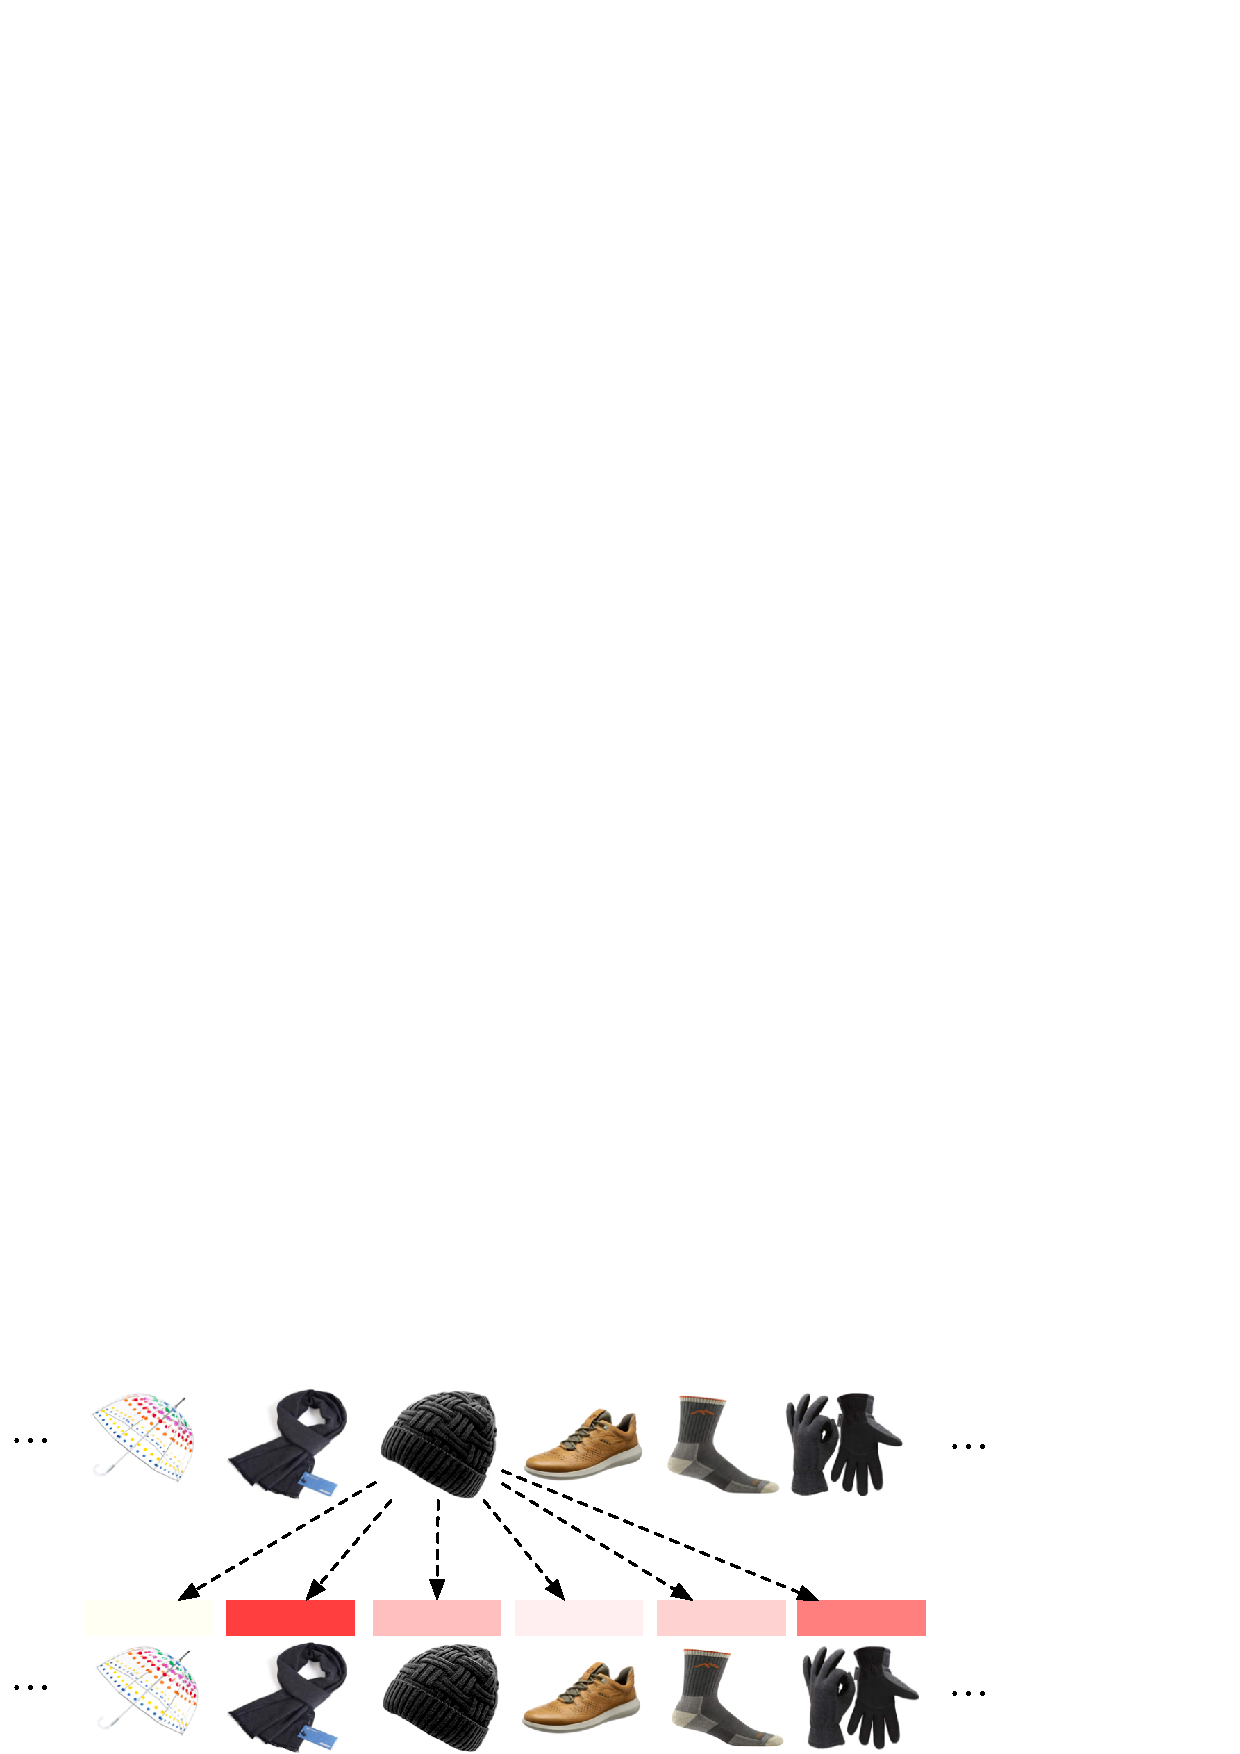
\includegraphics[width=1.0\columnwidth]{figure/attention.pdf}}
	\caption{Attention weight visualization. \textit{AtLocation} is required for prompt in the left column and \textit{PartOf} is required for prompt in the right column.} \label{fig:attention}
\end{figure}
Specifically, we focus on the attention weights between [MASK] token and 
other tokens in the prompt. A first glance of change of attention pattern 
is given in \figref{fig:LAMA} and we show more examples of other ConcetpNet 
relations in \figref{fig:attention}. We observe that while the original 
pretrained model tends to attend to special tokens like period and [SEP], 
the subnetwork successfully grasps the relevant concepts~(i.e., apple, 
worms, and basement) in the prompt hence produces the right object. 
We also use t-SNE~\citep{vanDerMaaten2008} to visualize the last layer's 
representation of [CLS] for each prompt. From \figref{fig:tsne}, the 
representations computed by original pretrained model are hardly separable as 
different types of knowledge are mixed together. In contrast, the pruned 
subnetwork can extract meaningful and disentangled representations for 
different commonsense relations.

\begin{figure}[th]
	\centering
	\scalebox{1.0}{\includegraphics[width=1.0\columnwidth]{figure/tsne_compare.pdf}}
	\caption{t-SNE visualization of [CLS]'s representation from original~(left) and pruned~(right) \textsc{BERT-base}.} \label{fig:tsne}
\end{figure}


\subsection{Commonsense Knowledge Base Completion~(CKBC)}
\label{sec:ckbc}
We evaluate the utility of identified relation-specific subnetworks on CKBC in an unsupervised manner. Specifically, we use the ConceptNet-100K benchmark provided by \citet{Li2016}. To ensure a fair evaluation, 
we manually create a subset of ConceptNet-100K 
consisting of triples with single-token subject/object. We also ensure that its dev/test set has \textbf{no overlap} with C-LAMA.
Each relation is associated with a sentence template~(provided in 
Appendix)~\citep{Kwon2019} of which the wording is distinct from 
those in C-LAMA. We acknowledge that these sentence templates might be suboptimal for certain relations, but prompt optimization is 
out of the scope of this paper. The resulting dataset contains 
$17,891$ training instances, $349$ development instances, 
and $446$ test instances.

\textbf{Link prediction.}~~We first formulate CKBC as a link prediction task 
and compare subnetworks~(i.e., $\mathcal{LM}_{\theta_r}$ 
is queried to predict missing link for instance of relation $r$) as well as original PLMs
against strong supervised KB completion mothods. 


\tabref{table:linkprediction} shows the results. Most of the supervised 
models outperform full-scale PLMs by a large margin, which suggests the 
inefficacy of directly using PLMs to perform link prediction. However, 
the subnetworks identified by our pruning procedure can
acquire performance on par with or better than state-of-the-art 
supervised models. Surprisingly, the pruned \textsc{DistilBERT} get the 
highest MRR, outperforming other larger and more advanced PLMs. 
\textsc{RoBERTa} struggles to predict correct objects, perhaps due to 
its larger vocabulary size compared to WordPiece~($50,265$ vs $30,522$) 
and less lexicon overlap~($53\%$ vs $59\%$) with the dataset.

%\KZ{It seems that our method (pruned models) don't work so well in the
%test set, compared to dev set. The scores for the same model between dev set and
%test set are also quite diff. Can you explain in this para?}

\textbf{Triple classification}~~We can also formulate CKBC as a triple classification task. Following ~\citet{Feldman2020}, we use estimated point-wise mutual information~(PMI) computed by pretrained language model as a surrogate of a triple's validity. An expectation-maximization-based Gaussian mixture clustering method is used and instances in the cluster with higher mean PMI are labeled as valid. 
\begin{table}[t]
	\centering
	\scriptsize
	\begin{tabular}{l|c}
		\toprule
		\textbf{Model} &  \textbf{F1 Score}\\
		\midrule
		\textsc{DistilBERT} & 74.1\\
		\textsc{DistilBERT}~(pruned) & \textbf{76.3}\\
		\midrule
		\textsc{BERT} & 73.7\\
		\textsc{BERT}~(pruned) & \textbf{76.7}\\
		\midrule
		\textsc{RoBERTa} &74.8 \\
		\textsc{RoBERTa}~(pruned) & \textbf{76.9}\\
		\midrule
		\textsc{MPNet} &76.5 \\
		\textsc{MPNet}~(pruned) & \textbf{78.0}\\
		\bottomrule
	\end{tabular}
	\caption{Triple classification on ConceptNet-100K.}
	\label{table:tripleclassification}
\end{table}
In our preliminary experiments, we found that the model pruned by the mask 
of a single relation might not be robust for PMI estimation and generally 
performed inferior to the intact model. 
In the same spirit as model ensembling, we then perform grid search over 
combinations of multiple knowledge, which is similar to what we did 
in zero-shot commonsense reasoning. For all four PLMs considered in 
\tabref{table:tripleclassification}, we observe that there exists one 
or multiple knowledge combinations delivering F1 score higher than the 
original models. 
%\KZ{Why is the difference between pruned and unpruned models
%not so big compared to link prediction?}

\textbf{Triple extraction.}~~We then investigate the ability of specialized 
subnetworks to extract novel commonsense knowledge triples absent 
from the dataset. We randomly sample 100 triples from the test set of 
ConceptNet-100K and for each sample use top-$K$ predictions from 
pruned \textsc{DistilBERT-base} as candidate objects. 
Three human annotators are asked to first determine the correctness of 
each candidate object and further determine their novelty~(i.e., not present 
in any of train/validation/test set) if deemed to be correct. 
The Fleiss Kappa inter-annotator agreement $\kappa$ is 0.66/0.65 
for precision and novelty, respectively.
\begin{figure}[t]
	\centering
	\scalebox{0.7}{\includegraphics[width=1.0\columnwidth]{figure/precision_novelty_2.pdf}}
	\caption{Precision-novelty curve with varied $K$.} \label{fig:extraction}
\end{figure}
\figref{fig:extraction} shows the change of precision-novelty with varied $K$. We observe a clear trade-off between the validity and novelty of triples extracted by the pruned model. As expected, a large $K$ inevitably makes noisy predictions but is more likely to extract unseen knowledge. For the purpose of knowledge enrichment, one might choose a large $K$ to ensure a desirable recall. We list the obtained novel triples in the Appendix D due to space limits.






\subsection{Commonsense Reasoning~(CSR)}
\label{sec:csr}
After identifying sparse subnetworks within PLMs that specialize in different commonsense knowledge, we now evaluate their generalization ability in the context of commonsense reasoning.
%One desirable outcome of our pruning procedure is the transformation from language representation to knowledge representation. We test if such subnetworks generalize in the context of commonsense reasoning.

\textbf{Many-shot learning.}~~We experiment with \textsc{BERT-base} and its deterministically pruned version using supervised fine-tuning on $7$ datasets: RTE~\citep{CambridgeJournals:6906264}, COPA~\citep{roemmele_choice_2011}, CommonsenseQA~\citep{talmor-etal-2019-commonsenseqa}, SWAG~\citep{zellers-etal-2018-swag}, HellaSWAG~\citep{DBLP:journals/corr/abs-1905-07830},   aNLI~\citep{DBLP:journals/corr/abs-1908-05739} and CosmosQA~\citep{huang-etal-2019-cosmos}. For each task, we identify the commonsense knowledge it might requires with a simple heuristic. Specifically, we obtain the five most frequent relations~(measured by how many times subject and object of certain relation appear in the context or answer) for each task and perform grid search over the combinations of these relationns. Then we take the union of masks for each relation and apply the resultant mask to the BERT as initialization for finetuning.
We repeat the training three times with different random seeds for each task. 
The  choice of mask combination for each task can be found in Appendix B.

The results in \tabref{table:finetuning} shows that, when initialized with proper weights, the model can be better fine-tuned on downstream commonsense reasoning tasks via more useful \textit{prior} knowledge. We further analyze the change of performance under the low-resource regime on COPA dataset. \figref{fig:copa} shows that the pruned \textsc{BERT} exhibits a notable advantage when training data is extremely scarce. As more training data is seen, the benefit of the pruned 
model becomes less prominent, i.e., $p>0.05$.
\begin{table}[t!]
	\centering
	\scriptsize
	\begin{tabular}{l|cc|c}
		\toprule
		\textbf{Task} & \textbf{Original} & \textbf{Pruned} &$p$-value \\
		\midrule
		RTE & 69.2$\pm${\scriptsize 2.3} & 69.8$\pm${\scriptsize2.0}& 0.12\\

		COPA & 62.4$\pm${\scriptsize 5.0} & 63.0$\pm${\scriptsize 4.7} &0.33  \\

		CommonsenseQA & 53.1$\pm${\scriptsize 0.6} & 54.1$\pm${\scriptsize 0.7} &0.08\\

		SWAG & 73.9$\pm${\scriptsize 0.3} & 74.2$\pm${\scriptsize 0.1} &0.09\\
		HellaSWAG & 38.9$\pm${\scriptsize 0.4} & 39.1$\pm${\scriptsize 0.5}&0.32  \\
		aNLI &63.7$\pm${\scriptsize 0.4} &64.0$\pm${\scriptsize 0.4}  &0.19\\
		CosmosQA &61.3$\pm${\scriptsize 1.0} &61.8$\pm${\scriptsize 0.2} &0.26\\
		\bottomrule
	\end{tabular}
	\caption{Finetuning results of \textsc{BERT} for CSR.}
	\label{table:finetuning}
\end{table}
\begin{figure}[t]
	\centering
	\scalebox{0.75}{\includegraphics[width=1.0\columnwidth]{figure/copa.pdf}}
	\caption{Finetuning result of \textsc{BERT} on COPA with varying portion of data.} \label{fig:copa}
\end{figure}
\begin{table*}[t!]
	\centering
	\scriptsize
	\begin{tabular}{l|cccccccc|c}
		\toprule
		\textbf{Model} &COPA-Tra. &COPA-Val. &CSQA &CA &WSC  &SM &ARCT1 &ARCT2 &Avg. \\
		\midrule
		\textsc{DistilBERT} &58.3 &60.0 &29.6 &84.6 &53.3  &71.6 &48.6 &50.4  &57.0  \\
		\textsc{DistilBERT}~(pruned) &\textbf{61.5} &\textbf{69.0} &\textbf{31.5} &\textbf{89.6} &\textbf{56.9}  &\textbf{72.1} &\textbf{53.4} &\textbf{51.6} & \textbf{60.7} \\
		\midrule
		\textsc{BERT} &60.2 &54.0 &26.5 &89.0 &57.3  &69.7 &46.8 &50.3 &56.7 \\
		\textsc{BERT}~(pruned) &\textbf{63.0} &\textbf{64.0} &\textbf{28.5} &\textbf{91.8} &\textbf{59.0}  &\textbf{71.7} &\textbf{50.0} &\textbf{52.0}  & \textbf{60.0}\\
		\midrule
		\textsc{RoBERTa} &60.7 &59.0 &39.9 &90.1 &61.8  &73.1 &48.6 &53.1 &60.7 \\
		\textsc{RoBERTa}~(pruned) &\textbf{65.3} &\textbf{72.0} &\textbf{40.4} &\textbf{93.4} &\textbf{62.9}  &\textbf{74.4} &\textbf{53.2} &\textbf{55.1} &\textbf{64.6}\\
		\midrule
		\textsc{MPNet} &66.5 &69.0 &40.0 &94.5 &64.3&75.8  &52.9 &56.7 &64.9  \\
		\textsc{MPNet}~(pruned) &\textbf{71.0} &\textbf{74.0} &\textbf{41.7} &\textbf{97.3} &\textbf{66.4}  &\textbf{77.5} &\textbf{56.1} &\textbf{57.7}  & \textbf{67.7}\\
		\bottomrule
	\end{tabular}
	\caption{Zero-shot results of accuracy~(\%) on commonsense reasoning tasks. Better results of each pair is in \textbf{bold}.}
	\label{table:zeroshot}
\end{table*}



\textbf{Zero-shot learning.}~~We next assess the ability of specialized 
subnetworks to perform zero-shot commonsense reasoning, a setting where 
the knowledge relied on to complete the task is solely determined by the model 
parameters. Here we focus on the following multiple-choice datasets: training set of COPA~(COPA-Tra.), validation set of COPA~(COPA-Val.), CommonsneseQA, Conjunction 
Acceptability~(CA)~\citep{Zhou2019}, 
Winograd Schema Challenge~(WSC)~\citep{levesque_winograd_2012}, 
SenseMaking~(SM)~\citep{wang-etal-2019-make}, 
ARCT1~\citep{habernal-etal-2018-argument} and 
ARCT2~\citep{DBLP:journals/corr/abs-1907-07355}. Each sample in the above datasets can be formulated as $\{[CLS]~context~[SEP]~choice_i ~[SEP]\}_{i=1}^{N}$, where $i$ is the subscript and $N$ is the number of choices. We compute the plausibility score of each choice using MLM head. Choice with the highest plausibility score is chosen as the answer. 

Since multiple types of knowledge are typically required for effectively 
reasoning over concepts, for each task, we perform grid search over 
combinations of $3$-$4$ different commonsense knowledge out of 
the $16$ total types and reported the best accuracy in \tabref{table:zeroshot}. 
We put the best combination for each model on each task in Appendix B
for space constraints. By combining multiple commonsense knowledge useful for the task, 
we show that the pruned models can actually surpass their full-scale 
version in all tasks considered in our experiments. 
The most likely explanation is that knowledge irrelevant to the specific task 
in the original models hurt the in-domain zero-shot reasoning capability. 
It also manifests that the most important reasoning skills vary from 
task to task.

\section{Conclusion}
We implement a novel sequence-based dependency parsing
framework which takes advantage of high order features 
in parsing history. 
%We can also adapt beam search to this framework so as to
%relax the strictly greedy nature. Vine pruning\cite{rush2012vine} could
%be incorporated to speed up the parsing.
More importantly, we discovered that the parsing accuracy is very sensitive to
the quality of parsing sequence. Future work can be focused on
developing better sequence predictors that outperform Malt action classifier.
Furthermore, we use two sets of features for sequence predictor and
head mapper right now. A unified set of features between these two components
are worth exploring.
%Besides, better sequence predicting method and unified feature
%representation of two components are worth exploring.
%
%Though we currently get a not bad result,
%the sequence predictor still needs more exploration.
%According to our experiment, slightly changes
%on the sequence can lead to a fatal decline on accuracy. Ensuring the match degree of training sequence and testing
%sequence demands a high quality of sequence predictor.
%
%Further, the features in our current implementation are not expanded and well tuned yet  and we are free to define high order features to make use of parsing history. Our framework is flexible to merge other technics to enhance the performance. Introducing beam could make up for our greedy decoder and improve our accuracy. Vine pruning\cite{rush2012vine} could speed up parsing process. Besides, better sequence predicting method and unified feature representation of two components are worth exploring.


%%%%%%%%%%%%%%%%%%%%%%%%%%%%%% 
%% 附录(章节编号重新计算,使用字母进行编号)
%%%%%%%%%%%%%%%%%%%%%%%%%%%%%% 
\appendix

% 附录中编号形式是"A-1"的样子
\renewcommand\theequation{\Alph{chapter}--\arabic{equation}}
\renewcommand\thefigure{\Alph{chapter}--\arabic{figure}}
\renewcommand\thetable{\Alph{chapter}--\arabic{table}}

%\include{body/app1} % 更新记录
%\include{body/app2} % 麦克斯韦方程
% \include{body/app3}


%%%%%%%%%%%%%%%%%%%%%%%%%%%%%% 
%% 文后(无章节编号)
%%%%%%%%%%%%%%%%%%%%%%%%%%%%%% 
\backmatter

% 参考文献
% 使用 BibTeX
% 包含参考文献文件.bib
\bibliography{reference/master}

%% 个人简历(学士学位论文没有个人简历要求)
% \include{body/resume}

% 致谢
\section*{Acknowledgements}
Thanks Yan Wang for insightful suggestions on the experiments.

% 发表文章目录
%%# -*- coding: utf-8-unix -*-
% !TEX program = xelatex
% !TEX root = ../thesis.tex
% !TEX encoding = UTF-8 Unicode
%%==================================================
%% pub.tex for SJTUThesis
%% Encoding: UTF-8
%%==================================================

\begin{publications}{99}
    \item\textsc{LUO K, LUO X, ZHU K}. {Inferring Binary Relation Schemas for Open Information Extraction}[C]// EMNLP: 2015: 555-560.
    \item\textsc{LUO K, LUO X, CHEN X}, et al. {A Data-driven Approach to Infer Knowledge Base Representation for Natural Language Relations}[C]// IJCAI: 2017:1174-1180.
    \item\textsc{LUO X, LUO K, CHEN X}, et al. {Cross-lingual Entity Linking for Web Tables}[C]// AAAI: 2018: 362-369.
    \item\textsc{LUO K, LIN F, LUO X}, et al. {Knowledge Base Question Answering via Encoding of Complex Query Graphs}[C]// EMNLP: 2018: 2185-2194.
    \item\textsc{LUO K, LU J, ZHU K}, et al. {Layout-aware Information Extraction from Semi-structured Medical Images}[J]. Computers in Biology and Medicine, 2019. (已录用)
\end{publications}


% 参与项目列表
%%# -*- coding: utf-8-unix -*-
% !TEX program = xelatex
% !TEX root = ../thesis.tex
% !TEX encoding = UTF-8 Unicode
%%==================================================
%% projects.tex for SJTUThesis
%% Encoding: UTF-8
%%==================================================

\begin{projects}{99}
    \item 参与自然科学基金中韩合作交流基金项目(2014年--2015年)
    %国科金外资助字第(61411140247)号 
    ``{多语言、跨文化语义联想概念网络的研究}''
    \item 参与自然科学基金面上项目(2014年--2017年)
    %61373031
    ``{基于动作概念的本体知识库及在文本处理上的应用}''
    %\item 973项目“XXX”
    %\item 自然基金项目“XXX”
    %\item 国防项目“XXX”
\end{projects}


%英文大摘要
%\include{body/bigabstract}

\end{document}
